% This is a copy version from https://github.com/thanhhungqb/thesis-template
% Please do not modified this project, when you want to start writing, make a clone of it for your own (Please read README.md)

\documentclass[12pt,a4paper,oneside]{book} % twoside for draf

%\usepackage{babel}
\usepackage[utf8]{vietnam}
\usepackage[utf8]{inputenc}
\usepackage[vietnamese,english]{babel}

\usepackage{tipa}
\usepackage{amssymb}
\usepackage{graphicx, wrapfig}
\usepackage{subcaption}
\usepackage{booktabs}
\usepackage{mathptmx}	% same Time New Roma
\usepackage{amsmath}
\usepackage{amssymb}
\usepackage{amsfonts}
\usepackage{sty/ipa}
%\renewcommand{\rmdefault}{phv} % Arial
%\renewcommand{\sfdefault}{phv} % Arial
\usepackage{array}
\newcolumntype{P}[1]{>{\centering\arraybackslash}p{#1}}
\newcolumntype{M}[1]{>{\centering\arraybackslash}m{#1}}
\usepackage{fancyhdr}
\usepackage{multirow}
\usepackage{algorithm2e}
\usepackage{hyperref}
\usepackage{float}
\usepackage{longtable}

\usepackage{sty/bkthesis}

% \usepackage[
% backend=biber,
% style=alphabetic,
% ]{biblatex}
% \addbibresource{refs.bib}

% To numbering figure continuously
\usepackage{chngcntr}
\counterwithout{figure}{chapter}
\counterwithout{table}{chapter}

\setlength{\parskip}{1em}
\renewcommand{\baselinestretch}{1.2}

\graphicspath{ {image/} }
\setcounter{secnumdepth}{2}
\crname{GRADUATION THESIS PROPOSAL}
% \ctname{NHẬN DIỆN VẬT THỂ TRONG ẢNH\\NHẬN DIỆN HƯỚNG NHÌN TRONG ẢNH}
\ctname{USING MACHINE LEARNING METHODS\\IN TRANSLATING SIGN LANGUAGE\\INTO VIETNAMESE}
\cstuname{
Student 1: Võ Tuấn Khanh (1810220)\\Student 2: Nguyễn Trí Nhân (1810390)}
\csSupervise{Assoc. Prof. Quản Thành Thơ}
\csReviewer{Dr. Nguyễn Đức Dũng}

\cttime{December 2021}

\thesislayout

\begin{document}
%-	Bìa cứng - màu xanh dương, chữ mạ vàng (xem mẫu đính kèm)
%-	Trang tên (tờ lót): chất liệu giấy, nội dung giống như bìa LV
%-	Ở gáy LV: in nhan đề LV (có thể in tóm tắt nếu nhan đề quá dài), size 15 – 17
%-	Phiếu Nhiệm vụ LV, chấm điểm Hướng dẫn & Phản biện (đã ký): nhận từ GVHD & GVPB sau khi bảo vệ (theo lịch hẹn).
%-	Lời cam đoan
%-	Lời cảm ơn/ Lời ngỏ
%-	Tóm tắt LV
%-	Mục lục
%-	Danh mục, bảng biểu, hình ảnh, ... (nếu có)
%-	Nội dung LV
%-	Danh mục TL tham khảo
%-	Phụ lục (nếu có)

\coverpage

\frontmatter


\begin{declaration}
	% ví dụ:

	% Nhận diện hướng nhìn trong ảnh (Nhận diện vật thể trong ảnh) không phải là một đề tài mới nhưng vẫn là một thách thức bởi: trong các ứng dụng: việc nhận diện hướng nhìn của con người qua hình ảnh đòi hỏi kết quả chính xác cao, ở Việt Nam, hiện tại không  thực sự có nhiều nghiên cứu chuyên sâu về đề tài. Trong quá trình nghiên cứu đề tài có rất nhiều kiến thức không nằm trong chương trình giảng dạy ở bậc Đại học tuy vậy chúng tôi xin cam đoan đây là công trình nghiên cứu của riêng tôi dưới sự hướng dẫn của tiến sĩ Nguyễn Đức Dũng. Nội dung nghiên cứu và các kết quả đều là trung thực và chưa từng được công bố trước đây. Các số liệu được sử dụng cho quá trình phân tích, nhận xét được chính tôi thu thập từ nhiều nguồn khác nhau và sẽ được ghi rõ trong phần tài liệu tham khảo.

  % Ngoài ra, tôi cũng có sử dụng một số nhận xét, đánh giá và số liệu của các tác giả khác, cơ quan tổ chức khác. Tất cả đều có trích dẫn và chú thích nguồn gốc.

  % Nếu phát hiện có bất kì sự gian lận nào, tôi xin hoàn toàn chịu trách nhiệm về nội dung luận văn của mình. Trường đại học Bách Khoa thành phố Hồ Chí Minh không liên quan đến những vi phạm tác quyền, bản quyền do tôi gây ra trong quá trình thực hiện.

We claim that this research is our work, conducted under the supervision and guidance of Associate Professor Quản Thành Thơ. The result of our research is authentic and has never been published in any way before. All the materials I utilized in this research were gathered from various sources and are referenced correctly in the references section. 

Furthermore, within this research, I also used the results of several other authors and organizations. All of them have been correctly cited. In any case of plagiarism, I stand by my actions and will be responsible for it. Therefore, Ho Chi Minh City University of Technology is not responsible for any copyright infringements conducted within our research.

\end{declaration}

\begin{acknowledgments}

To complete this thesis outline, I would like to express my deep gratitude to Associate Professor Quản Thành Thơ for his guidance throughout the research process.

We want to express our sincere thanks to the Faculty of Computer Science and Engineering teachers, Ho Chi Minh City University of Technology, for their dedication to imparting knowledge during our years of study at the school. The knowledge accumulated during the study process is the foundation for the research process and the luggage to enter life confidently.

Finally, I wish you good health and success in your noble career.
	
\end{acknowledgments}
	
\begin{abstract}

Presently, more than two million people with deaf and hard of hearing in Vietnam cannot talk freely with those who do not have those symptoms. There are a few ways for the deaf and hard of hearing to communicate with others, but they are ineffective and inefficient. The most used method is through notes or body language to express their thoughts to others. However, not many people know about sign language, making it hard to understand.

To help those people communicate more efficiently, we have built a system using Artificial Intelligence to translate sign language into Vietnamese. The design, in short, contains two physical modules, which are a camera and a smartphone having installed our application. Beneath the application is an Artificial Intelligence-based pipeline with six more submodules that translate sign language into text and read the word out loud through the phone’s built-in speaker.

Besides, the sign language data is collected from various resources through the site \url{https://tudienngonngukyhieu.com/}. Based on the videos that instruct vocabularies, we gathered and categorized them for the primary dataset of this system.

Overall, our system currently can translate some words. However, the more time it takes to learn the new terms, the more accurate the system is. The system can translate many more words with a much more extensive sign language library. We suppose our approach not only helps people with disabilities communicate and enrich their lives, but it also increases the volume of the workforce and reduces the economic burden on the national budget since then.

\end{abstract}	


\tableofcontents
% \listofsymbols
\listoffigures
\listoftables
%\listofalgorithms


\mainmatter

\fancyhead{}  % Clears all page headers and footers
%\rhead{\thepage}  % Sets the right side header to show the page number
%\lhead{}  % Clears the left side page header
%\fancyfoot[positions]{footer}
\renewcommand{\footrulewidth}{0.4pt}

\pagestyle{fancy}  % Finally, use the "fancy" page style to implement the FancyHdr headers
%

\chapter{Introduction}
	
\section{Problem statement}

"Each deaf person is a separate world, and they feel more self-deprecating and alone when they do not interact and share with others. They still have the desire to contribute to society", said Mr. Do Hoang Thai Anh, Vice Chairman of the Hanoi Deaf Association.

Language is a universal key that not only connects people but also builds up our society. Any disability that affects the ability to communicate is a significant disadvantage, especially for people with disabilities. They cannot integrate, have fun, learn, and communicate like ordinary people because they cannot express their thoughts, ideas, and desires to develop society as we do. That burden usually makes them fall into poverty, live a dependent life, and be exploited, apart from society. Hence, it is challenging for them to have beautiful lives.

In 2020, Vietnam had more than 2.5 million people who are deaf and mute, yet, only a tiny portion of them took part in education, had the chance to be understood, and integrated with society.

According to UNICEF, Households with members with disabilities are often poorer, children with disabilities are at risk of having less education than their peers, and employment opportunities for people with disabilities are also lower than those without disabilities. Even though people with disabilities are beneficiaries of the policy, and poverty is not a burden to accessing health facilities, very few people with disabilities (2.3\%) have access to functional rehabilitation services when being sick or injured. Besides, there still exist inequalities in living standards and social participation for people with disabilities [6]. Many organizations are founded to support, help, and create better living conditions for people with disabilities to develop. However, this work still has many difficulties and inadequacies as there is no formal school or class. Moreover, there is no specific profession for this group of people, and the number of translators who know sign language is insufficient, while they take an essential role in helping the people with disabilities connect with society.

A quote from Cavett Robert, "Life is a grindstone, and whether it grinds you down or polishes you up is for you and you alone to decide." However, it is challenging for these people to go to school and have an excellent education. They have their desires and dreams, but our resources and efforts are not enough to make them a polished grindstone. Furthermore, sign language shares the same property as any other spoken language; each different region and territory has a different way of expressing sign language. These unseen differences make communication, self-expression, and information exchange even more complex and challenging for humanity.

In short, we must admit that understanding and breaking the language barrier is extremely necessary and urgent because the deaf and mute, like many other ordinary people, deserve to be assisted, understood, and acknowledged. Furthermore, we believe our system is the resolve to problems of the deaf and hard of hearing.

\section{Goals of this thesis}

% Đề tài này hướng đến mục tiêu là nghiên cứu, hiểu và hiện thực một số giải pháp để có thể chuyển đổi từ ngôn ngữ ký hiệu sang tiếng Việt. Trong đó, hệ thống phải có khả năng thực hiện việc nhận video từ camera được gắn trên nón, thực hiện các giải thuật và xuất ra chữ trên màn hình điện thoại.
% 
% Từ mục tiêu tổng quát trên, tác giả sẽ lần lượt giải quyết các vấn đề sau để đưa ra một giải pháp thiết kế và hiện thực một kiến trúc hệ thống giải quyết được bài toán của đề tài:

This thesis aims to research, understand, and implement solutions to convert from sign language to Vietnamese. In particular, the system must receive a queue of images from the camera mounted on the hat, use the implemented algorithms to process and display text on the phone screen.

We can solve the above problem by breaking it down into smaller ones listed below. With each issue, we will give our solution and architect a system that can solve the whole problem of this thesis.
 
\begin{itemize}
	\item Search and collect data on sign language, conduct evaluation, classification, and normalization of data.
	\item Find out the approaches that have been implemented.
	\item Design architecture of the model
	\item Plan to implement, develop a sign language conversion system
	\item Build an application that users can utilize
\end{itemize}


\section{Scopes of this thesis}

% TLDR: In this case study, we will build a system including an app and camera module to translate at least 100 words from sign language into Vietnamese.

In this case study, we will build a system including an app and camera module to translate sign language into Vietnamese. Because of the limited time, the scope of the study is also limited as follows:

\begin{itemize}
	\item The system can only translate Vietnamese words
	\item The system can only recognize the words that it has been trained with
\end{itemize}

\section{Structure of this thesis proposal}

This proposal includes four sections and each will convey the related works and output when doing this thesis.

\begin{table}[H]
	\centering
	\begin{tabular}{ |c|p{13.5cm}| } 
		\hline
		Chapter          & Content                                                                                       \\
		\hline
		1                & A brief introduction about plan and objectives of thesis                                      \\
		\hline
		2                & Related works that had been done and how they help us in doing this thesis                    \\
		\hline
		\multirow{2}*{3} & Introduction of theoretical background as foundation knowledge that are applied in the thesis \\
		\hline
		4                & Solution and design approach for problem statement of this thesis                             \\
		\hline
		5                & Plan to finish this thesis in the upcoming time                                               \\
		\hline
		6                & Proposed chapters of the thesis                                                               \\
		\hline
		7                & Summary of this thesis proposal                                                               \\
		\hline
	\end{tabular}
	\caption{Structure of this thesis proposal}
\end{table}
\chapter{Related Work}
  Nowadays, Many scholars from all around the world have submitted research 
  projects relating to the topic of turning sign language into text, 
  using a variety of methodologies and perspectives.
  % TODO: Change paper
  In which, two main approaches can be mentioned as follows:
  \begin{itemize}
    \item Glove based approaches:
    With this approach, it requires deaf and mute people to wearing a sensor glove. When user
    has any different action or gesture, these sensor will be recorded. After that, data from
    sensor will analyze by analyzer component and return the output for user.
    \item Vision based approaches:
    With this approach, image processing algorithms will be applied to be able to determine
    hand position, gestures and movements of the hand. The user will not have to wear necessary
    equipment like glove based approaches, which is convenient for user. However, with using
    library or algorithms of image processing, we need to deal with worst quality output, which is
    greatly affected by this algorithms.
  \end{itemize}

  Early work, with vision based approach, they used several types of
  image processing algorithm to build a feature vectors base on a single RGB image of hand.
  In this paper "Real-time sign language recognition using a consumer depth camera" \cite{kuznetsova2013real},
  with using multi-layered random forest (MLRF), not only it allows they recognize hand signs
  correctly, but also minimize training time and effort. Or in this paper "Sign Language Translation in Urdu/Hindi Through
  Microsoft Kinect", sign language can be recognize by an auxiliary equipment: Microsoft Kinect (see figure \ref{fig:Chap2-MS-Kinect}), which captures
  the signs of the deaf person, after that, through the computer system, they can detect what does deaf people say.

  \begin{figure}[H]
    \centering
    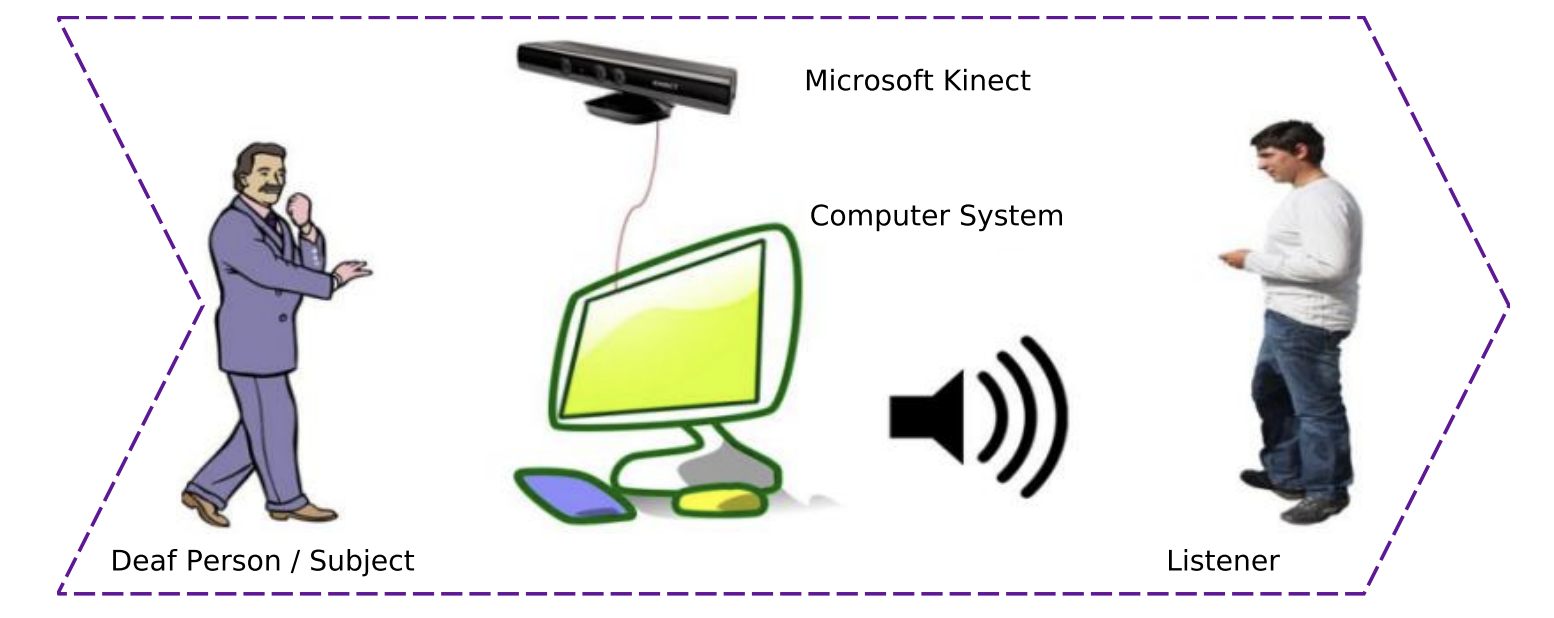
\includegraphics[width=\textwidth]{img/Chap2/MS-Kinect.png}
    \caption{Using Microsoft Kinect in translating sign language}
    \label{fig:Chap2-MS-Kinect}
  \end{figure}

  Beside vision based approach, glove based approach has many relevant research. This paper “The Language of Glove: Wireless gesture
  decoder with low-power and stretchable hybrid electronics” \cite{o2017language} introduces the way to convert American
  Sign Language (ASL) alphabet into text and display it on a computer 
  or smartphone (see figure \ref{fig:Chap2-Glove-Base}). With sensor glove, they can detect which hand gesture is
  performed and sent the result to smartphone via bluetooth. The sign language
  interprets into some text and displays on the digital display screen.
  Both this approach is useful in the real world for the deaf and dumb 
  who are unable to converse with normal people.

  \begin{figure}[H]
    \centering
    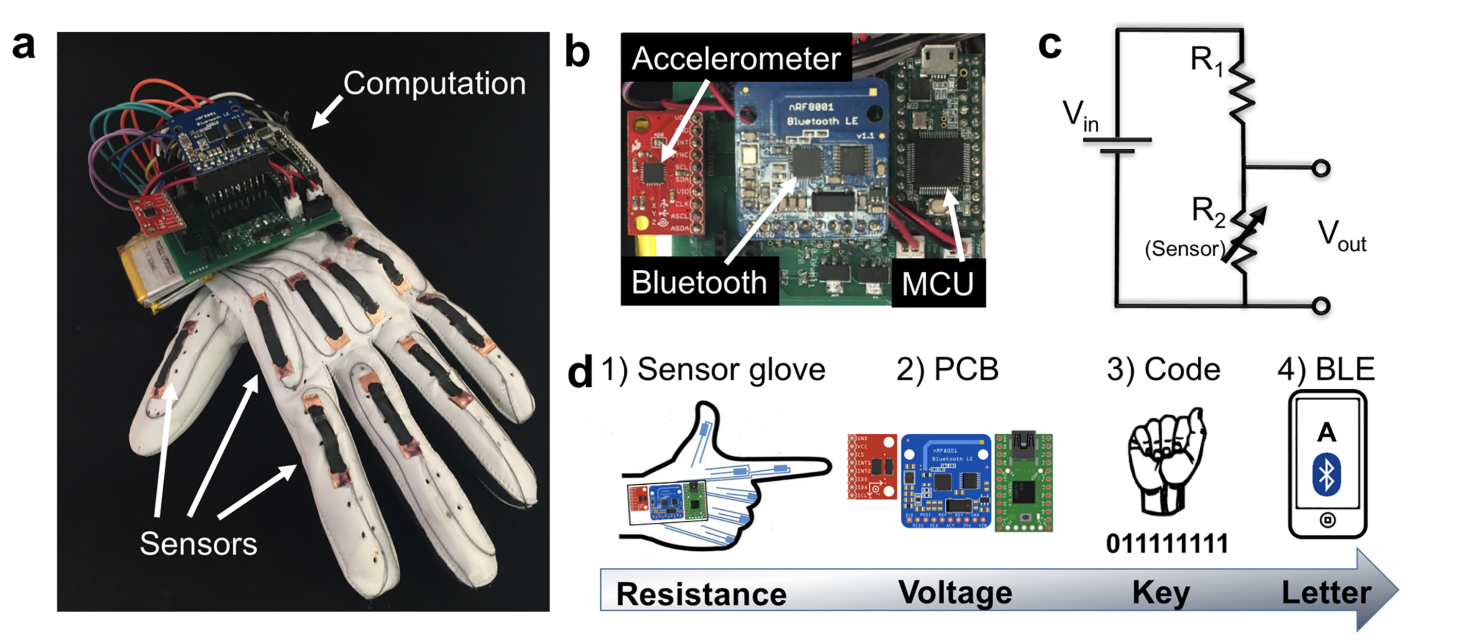
\includegraphics[width=\textwidth]{img/Chap2/Glove-Based.png}
    \caption{Glove based approach in translating sign language}
    \label{fig:Chap2-Glove-Base}
  \end{figure}

  % TODO: Fix grammar for this
  With both approaches above, it has some problems, that is, they can only recognize 
  a very small number of words, like an alphabet, number or some word with easily hand shape and no motion .
  However, in sign language, it not easy, there will be many words 
  that use the same hand shape but will differ in many characteristics, such as position 
  and direction. To our knowledge, there is currently no model that can handle the 
  conversion of sign language flexibly and conveniently for the deaf-mute, helping them 
  to communicate effectively and naturally. Therefore, by applying appropriate 
  technologies, the authors carry out this graduation thesis with the goal of breaking down 
  the barriers between deaf-mute people and normal people, helping them to become self-sufficient. 
  more confident in daily communication.


\chapter{Theoretical Background}

\section{Convolution Neural Network - CNN}

Convolution Neural Networks are a particular class of Neural Networks \cite{masood2018real}. They are made up of neurons that have learnable weights and biases. Each neuron receives some inputs, performs a dot product, and optionally follows it with a non-linearity. CNN mainly consists of Convolution Layers, Pooling Layers, Activation Layers, and Fully Connected Layers. ConvNet architectures make the explicit assumption that the inputs are images, which allows us to encode specific properties into the architecture. These then make the forward function more efficient to implement and vastly reduce the number of parameters in the network. Some of the primary uses of CNN can be mentioned as image classification, object detection, semantic segmentation, face recognition, ...

%Insert picture about CNN https://scholarworks.iupui.edu/bitstream/handle/1805/24768/FINAL%20Prasham_Shah_Thesis%20.pdf?sequence=1&isAllowed=y
\begin{figure}[H]
	\centering
	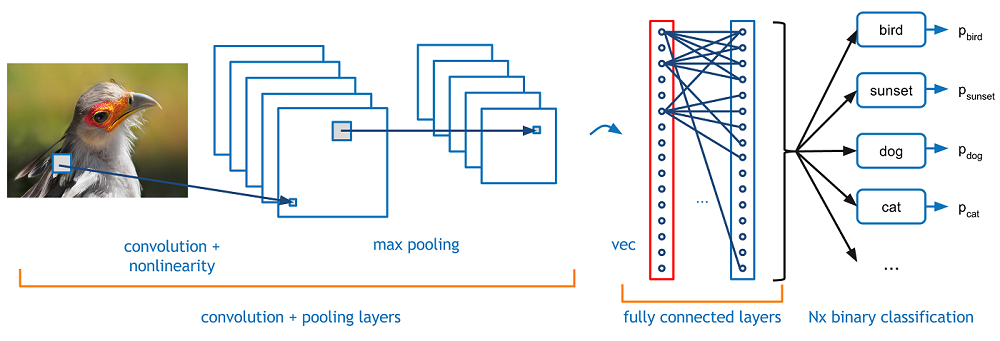
\includegraphics[width=\textwidth]{img/Chap3/Cover.png}
	\caption{Convolution Neural Network}
	\label{fig:Chap3-OverviewTheCNN}
\end{figure}

The figure \ref{fig:Chap3-OverviewTheCNN} above shows an example of a convolution neural network, which is taking an image as input and then extracting features from it through various layers and then finally predicting the class of the object in the given image.

\subsection{Architecture}

Convolution Neural Networks have a different architecture than regular Neural Networks, and we can see this difference in figure \ref{fig:Chap3-DiffArchCNN_NNN} below. Regular Neural Networks transform an input through a series of hidden layers. Every layer comprises a set of neurons, where each layer is fully connected to all neurons in the previous layers. Finally, a last fully-connected output layer represents the predictions with CNN architecture. First of all, the layers are organized into three dimensions: width, height, and depth. Further, the neurons in one layer do not connect to all the neurons in the next layer but only to a small region. Lastly, the system will reduce the final output to a single vector of probability scores, organized along the depth dimension.

%FIXME: Insert image of diff architecture : https://www.freecodecamp.org/news/an-intuitive-guide-to-convolutional-neural-networks-260c2de0a050/
\begin{figure}[H]
	\centering
	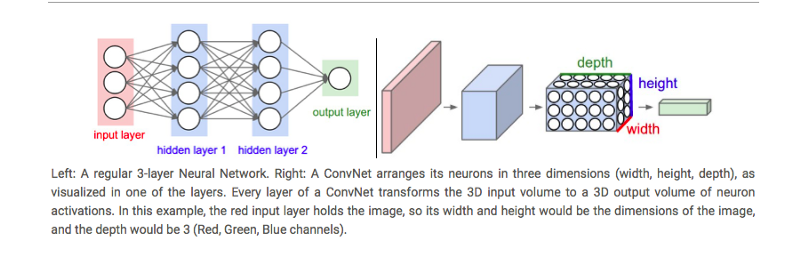
\includegraphics[width=\textwidth]{img/Chap3/DiffArchCNN-ANN}
	\caption{Different between Normal Neural Network and Convolution Neural Network}
	\label{fig:Chap3-DiffArchCNN_NNN}
\end{figure}

%FIXME: Insert image of CNN arc: https://www.freecodecamp.org/news/an-intuitive-guide-to-convolutional-neural-networks-260c2de0a050/
\begin{figure}[H]
	\centering
	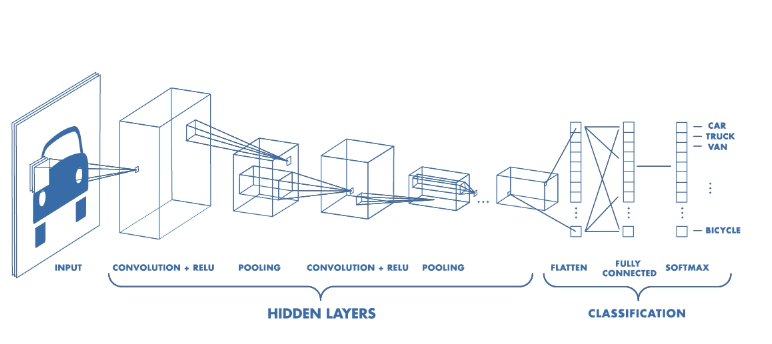
\includegraphics[width=\textwidth]{img/Chap3/CNN-Arch}
	\caption{Convolution Neural Network Architecture}
	\label{fig:Chap3-CNN_Arch}
\end{figure}

As we can see in figure \ref{fig:Chap3-CNN_Arch}, CNN can be divided into two parts:
\begin{enumerate}
	\item The hidden layers/ Feature extraction part\\
	In this part, the network will perform a series of convolutions and pooling operations during which the features are detected. If you had a picture of a zebra, this is the part where the network would recognize its stripes, two ears, and four legs.
	\item The Classification part\\
	The fully connected layers will serve as a classifier on top of their extracted features. They will assign a probability for the object on the image being what the algorithm predicts it is.
\end{enumerate}

\subsection{Feature extraction part}
\subsubsection{Convolutional Layer}

The convolution layer is the core building block of a Convolutional Network that does most of the computational heavy lifting. A convolution is executed by sliding the filter over the input. At every location, matrix multiplication is performed and sums the result onto the feature map. This extracting features from images happen throughout the CNN's convolutional layers. This process is illustrated in figure \ref{fig:Chap3-CNN_Layer}

% FIXME: https://scholarworks.iupui.edu/bitstream/handle/1805/24768/FINAL%20Prasham_Shah_Thesis%20.pdf?sequence=1&isAllowed=y
\begin{figure}[H]
	\centering
	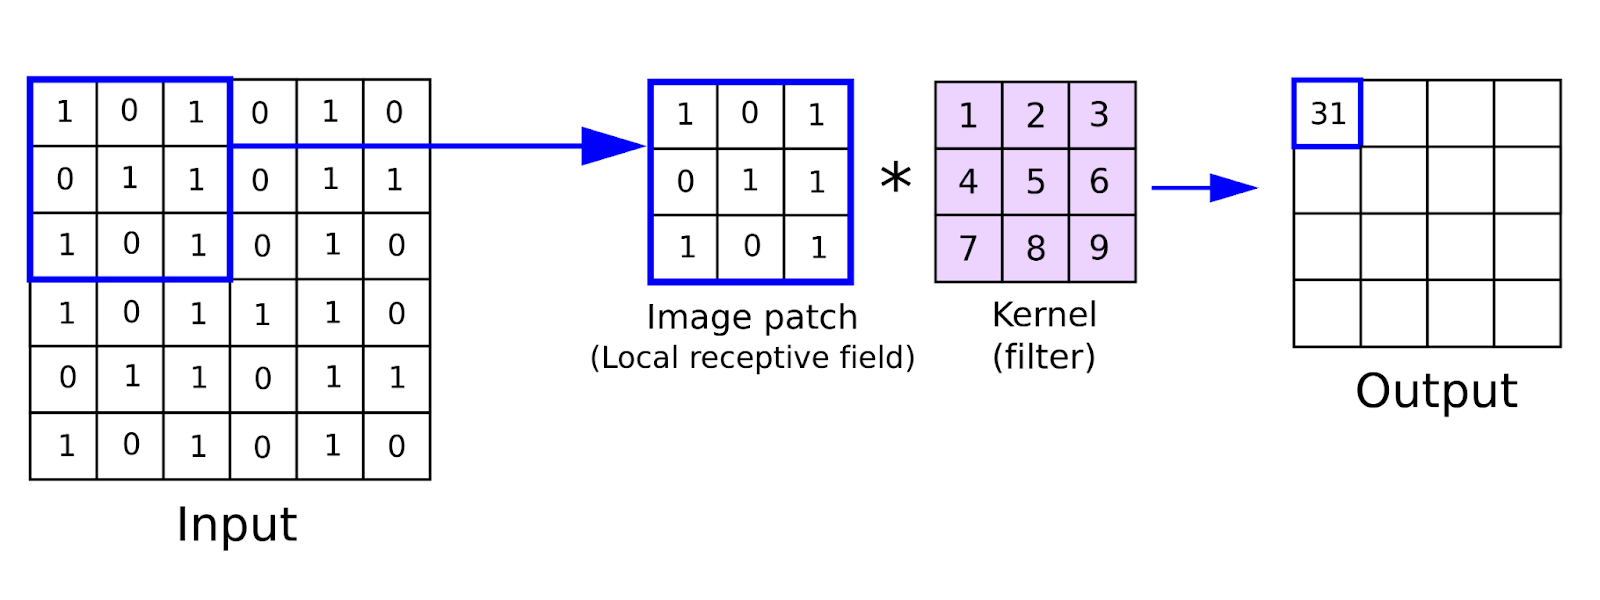
\includegraphics[width=\textwidth]{img/Chap3/ConvLayer}
	\caption{Convolution Neural Network Layer}
	\label{fig:Chap3-CNN_Layer}
\end{figure}

When the feature map is made, we can pass each value in the feature map through a non-linearity function, such as ReLU, sigmoid before it becomes the input of the next convolution layer.

Due to the size of the feature map being always smaller than the input, we have to do something to prevent our feature map from shrinking. This is where we use padding (\ref{fig:Chap3-CNN_Padding}). A layer of zero-value pixels is added to surround the input with zeros so that our feature map will not shrink. In addition to keeping the spatial size constant after performing convolution, padding also improves performance and ensures the Kernel and stride size will fit in the input.

% FIXME: => Need picture
\begin{figure}[H]
	\centering
	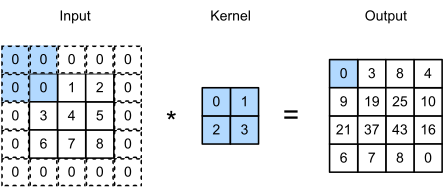
\includegraphics[width=\textwidth]{img/Chap3/CNN_Padding}
	\caption{Using padding for strike one in Convolution Layer}
	\label{fig:Chap3-CNN_Padding}
\end{figure}
\subsubsection{Pooling Layers}

After a convolution layer, it is common to add a pooling layer in between CNN layers. The function of Pooling is to continuously reduce the dimensionality to reduce the number of parameters and computation in the network. This action shortens the training time and controls overfitting.

There are mainly two types of Pooling Layers in a CNN: Max Pooling and Average Pooling. The functionality of these two types of layers is demonstrated in figure \ref{fig:Chap3-CNN_Pooling}. Max Pooling restores the maximum value from the picture segment covered by the Kernel. Average Pooling converts the average values from the bit of the picture surrounded by the Kernel.

\begin{figure}[H]
	\centering
	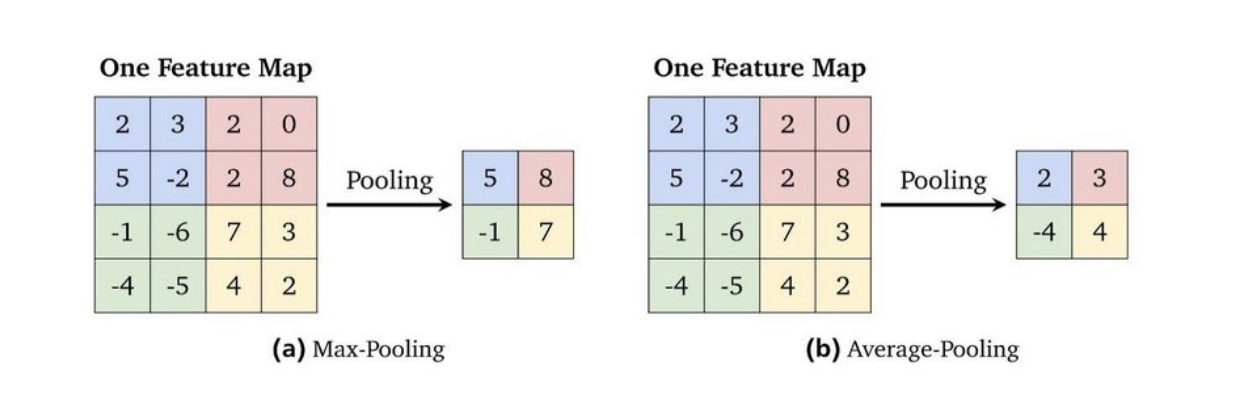
\includegraphics[width=\textwidth]{img/Chap3/Pooling}
	\caption{Max Pooling and Average Pooling}
	\label{fig:Chap3-CNN_Pooling}
\end{figure}

% FIXME: Insert image about max pooling and average pooling

\subsubsection{Activation Layers}

In general, Neural networks and CNNs rely on a non-linear "trigger" function to signal distinct identification of likely features on each hidden layer. CNN may use a variety of specific functions (figure \ref{fig:Chap3-CNN_ActiveFunction}), such as rectified linear units (ReLUs) and continuous trigger (non-linear) functions—to efficiently implement this non-linear triggering.

\begin{figure}[H]
	\centering
	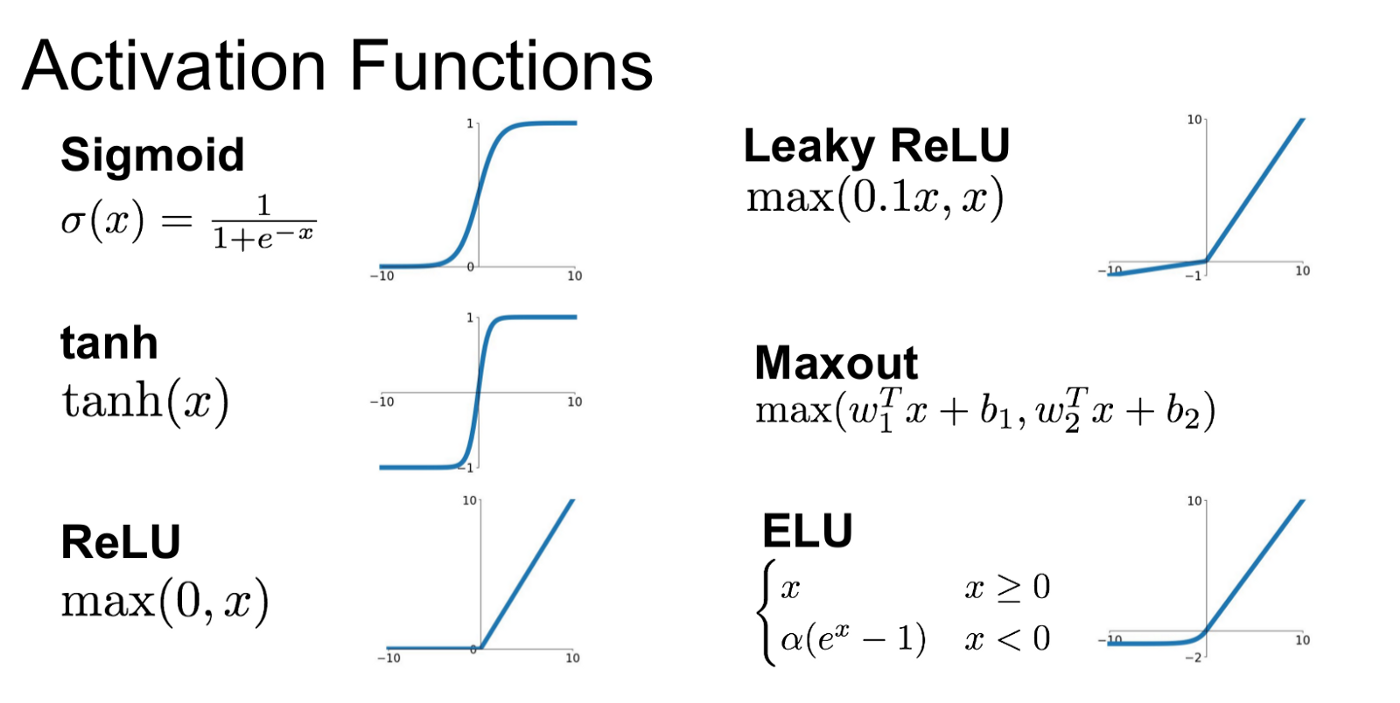
\includegraphics[width=\textwidth]{img/Chap3/ActiveFunction}
	\caption{ Some Active Function common used in CNN }
	\label{fig:Chap3-CNN_ActiveFunction}
\end{figure}
% FIXME: Insert picture of some function like ReLU, tanh ....
\subsection{Classification part}
\subsubsection{Fully connected layers}

The last layers of a CNN are fully connected. Neurons in a fully connected layer have complete connections to all the activations in the previous layer. This part is, in principle, the same as a regular Neural Network.

Figure \ref{fig:Chap3-FC} illustrates the way of input value stream into the fully connected layer. Because these fully connected layers can only accept one-dimensional data, we need to convert our 3D data to 1D data. After passing through some FC, we will get the data classification result.

\begin{figure}[H]
	\centering
	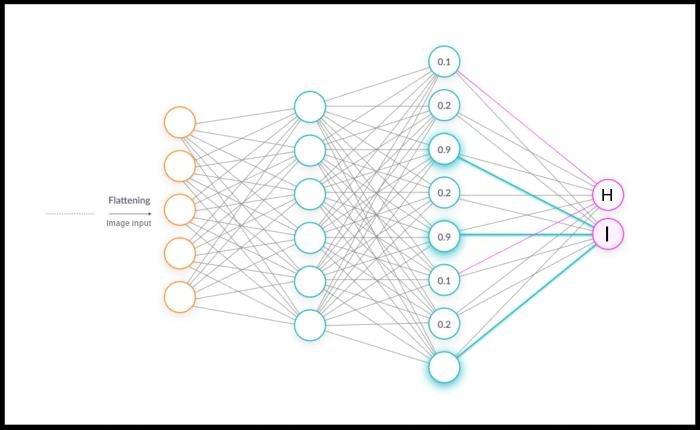
\includegraphics[width=\textwidth]{img/Chap3/FC}
	\caption{ Fully connected Layer}
	\label{fig:Chap3-FC}
\end{figure}
% FIXME: Insert picture ...
\section{Media Pipe}\label{sec:MediaPipe}
% FIXME: Lấy từ eureka bỏ vào
\subsection{Introduction to Media Pipe Hands}
MediaPipe Hands (\ref{fig:Chap3-MediaPipe}) is a high-resolution tracking system for hands and fingers \cite{zhang2020mediapipe}. It uses machine learning to infer 21 3D hand landmarks from a single frame. This solution delivers real-time performance on a cell phone and even scales to many hands, whereas current state-of-the-art systems rely primarily on powerful desktop environments for inference.

\begin{figure}[H]
	\centering
	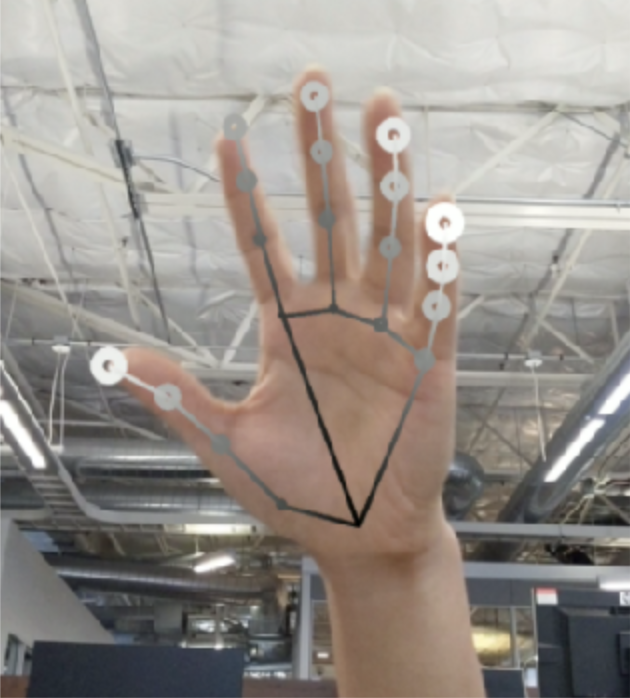
\includegraphics[width=0.8\textwidth]{img/Chap3/Media Pipe}
	\caption{ Media Pipe real time tracking 3D hand landmarks}
	\label{fig:Chap3-MediaPipe}
\end{figure}

MediaPipe Hands makes use of a machine learning pipeline that consists of several models that work together: A palm detection model, which acts on the entire image, will return an orientated hand bounding box. A hand landmark model that returns high-fidelity 3D hand key points from the cropped image region determined by the palm detector.

However, providing the hand landmark model with a correctly cropped hand image minimizes the requirement for data augmentation drastically (such as rotations, translations, and scaling) and instead allows the network to focus on coordinate prediction accuracy. Furthermore, in this ML pipeline, crops can be created based on the hand landmarks recognized in the previous frame, and palm detection is only used to localize the hand when the landmark model can no longer detect its presence.
\subsection{Palm detection model}
The Media Pipe team provides the palm detection model to detect initial hand locations and distinguish whether the hand recognized is left or right, which is very useful as each sign goes along with a different side will result in different meanings. They created a single-shot detector model, comparable to the face detection model in MediaPipe Face Mesh \cite{MediaPipeFaceMesh}, tailored for mobile real-time applications. Hand detection is difficult: our model must detect occluded and self-occluded hands and work across many hand sizes with a significant scale span relative to the image frame.

According to their statement, the methods they use to address the above challenges vary in many strategies. First, instead of training a hand detector, they train a palm detector because estimating bounding boxes of inflexible objects like palms and fists is much easier than recognizing hands with articulated fingers. Furthermore, the non-maximum suppression method performs effectively even in two-hand self-occlusion situations such as handshakes because palms are small objects. Furthermore, palms can be simulated using square bounding boxes (anchors in ML language) that ignore other aspect ratios, reducing 3-5 anchors. Second, even for tiny objects, an encoder-decoder feature extractor is used for more extensive picture context awareness (similar to the Retina Net approach). Finally, the significant scale variance limits focus loss during training to support many anchors.

Using the strategies described above gives an average precision of 95.7 percent in palm detection. With no decoder and a regular cross-entropy loss, the baseline is just 86.22 percent.

\subsection{Hand landmark model}
Following palm detection over the entire image, our next hand landmark model uses regression to accomplish exact key point localization of 21 3D hand-knuckle coordinates (see figure \ref{fig:Chap3-HandLandMark}) within the detected hand regions, i.e., direct, coordinate prediction. Even with partially visible hands and self-occlusions, the model develops a consistent internal hand posture representation.
\begin{figure}[H]
	\centering
	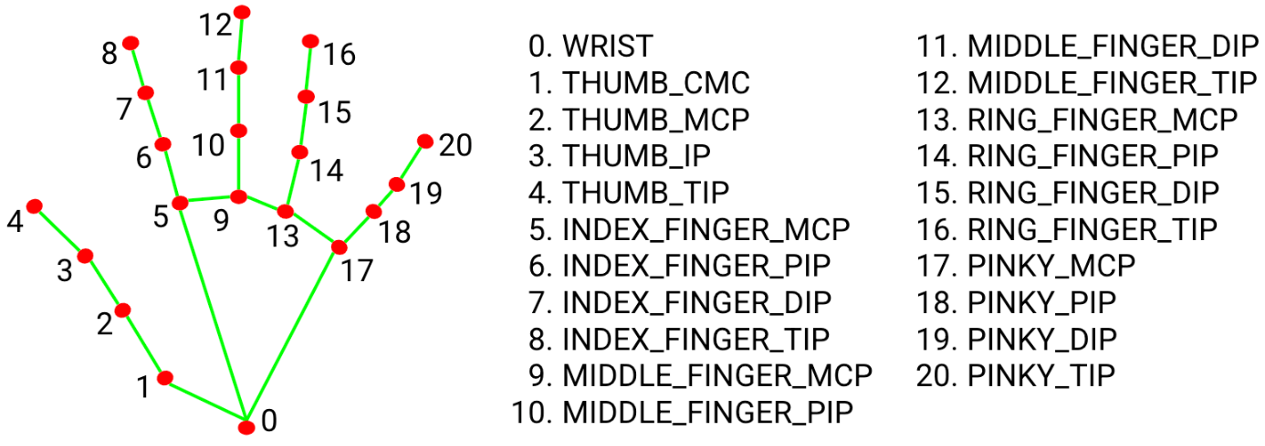
\includegraphics[width=\textwidth]{img/Chap3/HandLandMark}
	\caption{ 21 Hand Landmarks }
	\label{fig:Chap3-HandLandMark}
\end{figure}


\section{Distance Matrix}

A distance matrix \cite{DistanceMatrix} is a table that shows the distance between pairs of objects. For example, in the figure \ref{fig:Chap3-DM}., we can see the length between A and B is 16, B and C is 37, and so on. In the diagonal of the table is the distance to the object from itself, so the value, as we can see, is 0. Distance matrices are sometimes called dissimilarity matrices.

\begin{figure}[H]
	\centering
	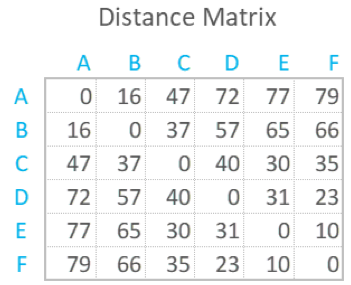
\includegraphics[width=0.6\textwidth]{img/Chap3/DM}
	\caption{ Distance Matrix }
	\label{fig:Chap3-DM}
\end{figure}

% FIXME: Insert picture of distance matrix

\subsection{Create Distance Matrix}

A distance matrix is computed from a raw data table. In the example below (figure \ref{fig:Chap3-DM_Formula}), we can use high school math (Pythagoras) to work out the distance between A and B.

% FIXME: Chèn công thức vào đây
\begin{figure}[H]
	\centering
	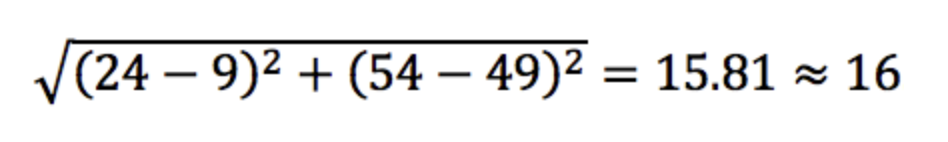
\includegraphics[width=0.7\textwidth]{img/Chap3/DM_Formula}
	\caption{ Calculating distance between A and B}
	\label{fig:Chap3-DM_Formula}
\end{figure}

We can use the same formula with more than two variables, known as the Euclidean distance. As a result, we have the distance matrix represented like figure \ref{fig:Chap3-DM-Raw}.

% FIXME: chèn bảng kết quả vào
\begin{figure}[H]
	\centering
	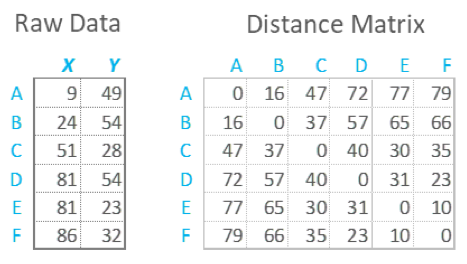
\includegraphics[width=0.7\textwidth]{img/Chap3/DM-Raw}
	\caption{ The Distance Matrix is constructed from Raw Data }
	\label{fig:Chap3-DM-Raw}
\end{figure}

\section{Beam search and Connectionist Temporal Classification}
% CheckList:
%   [x] BeamSearch
%   [x] CTC recap
%   [x] Combination
%   [x] Pseudo code
\subsection{Connectionist Temporal Classification}

Connectionist Temporal Classification (CTC) \cite{hannun2017sequence} is a type of Neural Network output helpful in tackling sequence problems like handwriting (figure \ref{fig:Chap3-Overview-CTC}) and speech recognition where the timing varies. Using CTC ensures that one does not need an aligned dataset, which makes the training process
more straightforward.

% FIXME: Insert about CTC in speech recognition
\begin{figure}[H]
	\centering
	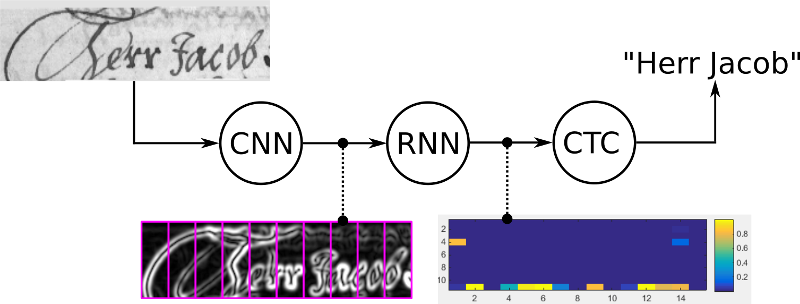
\includegraphics[width=\textwidth]{img/Chap3/Overview-CTC}
	\caption{ Overview of a Neural Network for handwriting recognition }
	\label{fig:Chap3-Overview-CTC}
\end{figure}

\subsection{Why we want to use CTC}

In the context of handwritten recognition, we could create a dataset with images of text-lines, and then specify for each horizontal position of the image the corresponding character as shown in figure \ref{fig:Chap3-Annottion-image-CTC} Then, we could train a model to output a character-score for each horizontal position. However, there are two problems with this solution.

\begin{itemize}
	\item It takes much time, and annotating the dataset at the character level is tiresome.
	\item What if the character takes up more than one time-step ?. We could get "tooo" because the "o" is a wide-character as shown in figure \ref{fig:Chap3-Annottion-image-CTC}. We must remove all duplicate characters like "t" and "o".
\end{itemize}

% FIXME: Insert image ...
\begin{figure}[H]
	\centering
	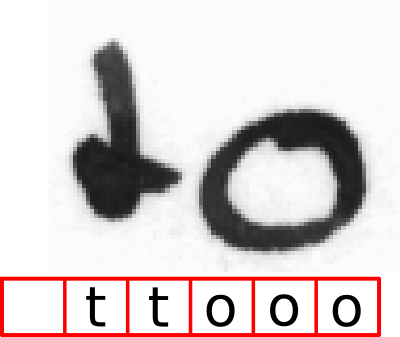
\includegraphics[width=0.6\textwidth]{img/Chap3/Annotation-image-CTC}
	\caption{ Annotation for each horizontal position of the image }
	\label{fig:Chap3-Annottion-image-CTC}
\end{figure}

CTC can solve both problems for us:
\begin{itemize}
	\item We can ignore both the position and width of the character in the image and only requires the text that occurs in the picture.
	\item Using decode techniques, we can directly get the result of the network, and no further post-processing of the recognized text is needed.
\end{itemize}

\subsection{Beam Search with CTC decoder}
CTC has more than the Decoding phase, it can have the Encoding, Loss calculation, but we don't need it in this graduation thesis scope anymore. So, here, we only mention to CTC decoder, but in the way, it combines with Beam Search \cite{scheidl2018word}. Because CTC in decoding context can connect with another algorithm like best-path decoding, ...

\subsubsection{Beam search}

In computer science, beam search \cite{BeamSearch} is a heuristic search algorithm that explores a graph by expanding the most promising node in a limited set. Beam search is an optimization of best-first search the reduces its memory requirements. Best-first search is a graph search that orders all partial solutions (states) according to some heuristic. But in beam search, only a predetermined number of the best partial solutions are kept as candidates. Pseudocode for the basic version of beam-search is shown in figure \ref{fig:Chap3-Basic-Version-BeamSearch}

\begin{figure}[H]
	\centering
	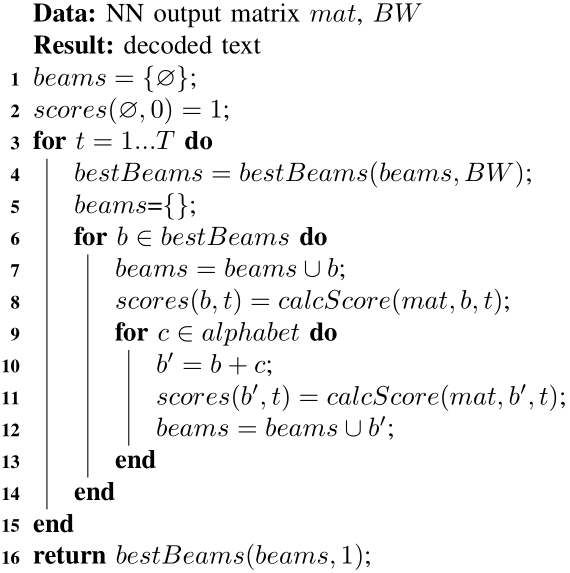
\includegraphics[width=0.8\textwidth]{img/Chap3/Basic-Version-BeamSearch}
	\caption{ Basic version of Beam Search }
	\label{fig:Chap3-Basic-Version-BeamSearch}
\end{figure}

% FIXME: Insert image about pseudo-code for beam-search

The beam search algorithm will be implemented through the following steps, with two parameters will be included: output matrix and beam width (BW), which specifies the number of beams to keep. First, the beam list and corresponding score are initialized (lines 1 and 2). After that, from 3-15, the algorithm will loop over all time-steps of the matrix output. At this point, only the best scoring beams (equal BW) from the previous time-step are kept (line 4). For each beam, we calculate the score and get a result (line 8); we will cover this step in more detail later. Further, each beam is extended by all possible characters from the alphabet (line 10), and again, a score is calculated (line 11). After the last time-step, the best beams are returned (line 16).

% FIXME: Insert image about beam search

\begin{figure}[H]
	\centering
	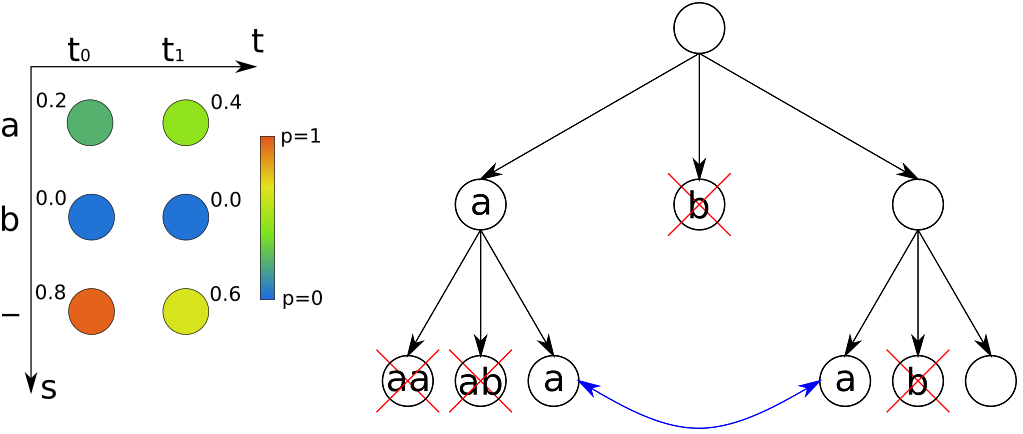
\includegraphics[width=\textwidth]{img/Chap3/BeamSearchTree}
	\caption{ NN output and tree of beams with alphabet = {"a", "b"} and BW = 2 }
	\label{fig:Chap3-BSTree}
\end{figure}

As we can see, in figure \ref{fig:Chap3-BSTree}, both output matrix to be decoded, and the tree of beams is shown. Beam search algorithm extended as possible and keep exactly BW candidates. Finally, we finished the last iteration, and the final step of the algorithm is to return the beam with the highest score, which is "a" in this example.

\subsubsection{Calculating the score}

As discussed above, in this part, we will talk about how to score the beam. We will split the beam-score into the score of paths ending with a blank(e.g. 'aa-') and paths ending with non-blank (e.g. 'aaa').

\begin{itemize}
	\item We denote the probability of all paths ending with a blank and corresponding to a beam b at time-step t
	      by $ P_{b}(b,t) $ and by $ P_{nb}(b,t) $ for the non-blank case.
	\item The probability $P_{tot}(b,t)$ of a beam b at time-step t is simply the sum of $P_b$ and $P_{nb}$, for example:
	      $P_{tot}(b,t) = P_b(b,t) + P_{nb}(b,t)$
\end{itemize}

\begin{figure}[H]
	\centering
	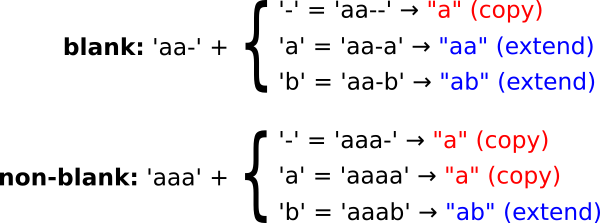
\includegraphics[width=0.7\textwidth]{img/Chap3/CTC_Scoring}
	\caption{ The effect of appending a character to paths ending with blank and non-blank }
	\label{fig:Chap3-CTC_Scoring}
\end{figure}

In figure \ref{fig:Chap3-CTC_Scoring}, we will see what happens when we extend a path. Three main case we can mention
is:
\begin{itemize}
	\item Extend by blank ('a' + '-' = 'a-')
	\item Extend by repeating last character ( 'aa' + 'a' = 'aaa' or 'aa-' + 'a' = 'aa-a')
	\item Extend by some other character ('aa' + 'b' = 'aab')
\end{itemize}

% FIXME: Viết lại các công thức bên dưới
And when we collapse the extended paths, two result we will get and some case we needed to handle:
\begin{itemize}
	\item The unchanged (copied) beam ('a' $ \rightarrow $ 'a'):
	      \begin{itemize}
		      \item To copy a beam, we can extend corresponding paths by a blank and get
		            paths ending with a blank: $ P_b (n, t) += P_{tot}(b, t-1)*mat(blank, t) $
		      \item Beside, with non-blank ending paths case, if we extend it by the last
		            character (the beam is not empty): $ P_{nb}(b,t) += P_{nb}(b,t-1)*mat(b[-1],t) $
		            with -1 indexes the last character in the beam
	      \end{itemize}
	\item An extended beam ('a' $\rightarrow$ 'aa' or 'ab'):
	      \begin{itemize}
		      \item To extend a beam. With the last character is different from the character we need
		            to extend, then there is no need for separating blanks ('-') in the paths:
		            $ P_{nb}(b+c,t) += P_{tot}(b,t-1)*mat(c,t) $
		      \item Or the last character of beam is repeated, we must ensure that the paths
		            end with a blank: $ P_{nb}(b+c,t) += P_b(b,t-1)*mat(c,t) $
		      \item We don't need t care about $P_b(b+c,t)$ because we added a non-blank character
	      \end{itemize}
\end{itemize}

\subsubsection{Putting it all together}

Figure \ref{fig:Chap3-BS_CTC} depicts the CTC beam search algorithm. It is similar to the basic version previously displayed. However, it includes the code to score the beams: copied beams (lines 7-10) and extended beams(lines 15-19). Finally, when looking for the best scoring beams, the programs rank them according to Ptot (line 4) and then take the BW best ones.

\begin{figure}[H]
	\centering
	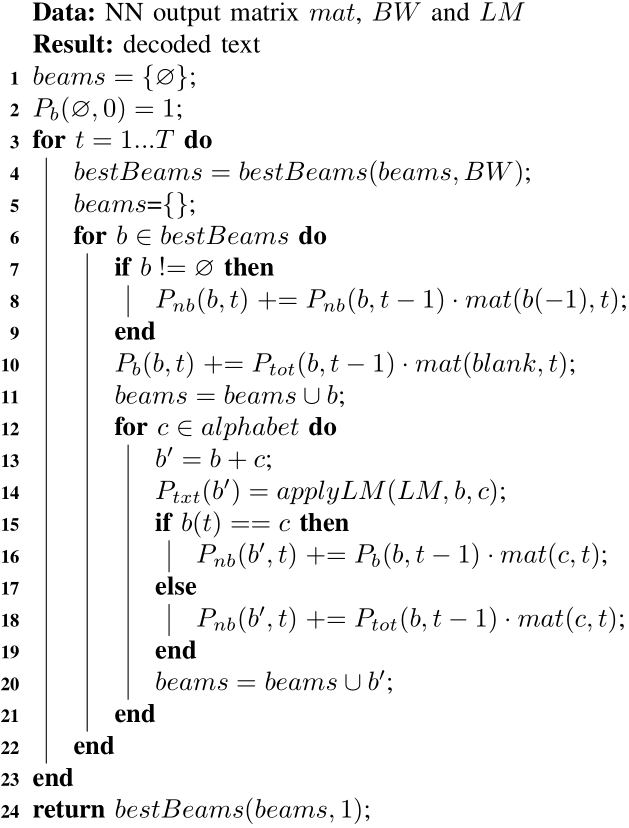
\includegraphics[width=0.8\textwidth]{img/Chap3/BS_CTC}
	\caption{ CTC beam search }
	\label{fig:Chap3-BS_CTC}
\end{figure}

\section{Technology}
%FIX-ME: Chém gió thêm ra phần này, sử dụng ngôn ngữ gì bla bla 
% Ứng dụng được viết bằng react-native. Sử dụng hệ thống authenticate của firebase
Overall the product application is developed with the technologies including java for android app and system authentication of Firebase.

\subsection{React Native}

\begin{figure}[H]
	\centering
	
\includegraphics[width=0.7\textwidth]{img/technology/ReactNative.png}
	\caption{React Native Logo}
	\label{fig:ReactNativeLogo}
\end{figure}

Traditional mobile app development necessitates knowledge of two distinct platforms (and programming languages): Android and iOS. However, using React Native\cite{ReactNative}, developers can create hybrid apps that operate on both platforms. The advantages of applying React Native in the app development process contain the following points.

\begin{itemize}
	\item \textbf{Cross-Platform}: One of the significant advantages of React Native is that we can write the same code for both the Android and iOS ecosystems simultaneously, with just minor changes for each platform.
	\item \textbf{One programming language}: There is no need to be familiar with the languages used for platform-specific application development because React Native employs JavaScript, which is currently one of the most popular programming languages\cite{10MostPopularProgrammingLang}. To be more specific, in this project, we use an advanced version of JavaScript, which is known as TypeScript, and we will discuss it in the later section.
	\item \textbf{Performance}: Because both platforms use the same code, React Native allows for the rapid creation of mobile applications. It also has a hot reloading functionality that ensures that modest changes to the program are shown to the developer right away.
\end{itemize}

Therefore, using this React Native framework benefits us in developing the same app for iOS devices from Apple Inc. According to the plan that we came up with before, when the product app works acceptably on Android devices, we will expand it and make it work on those iOS devices without massive effort when translating an app from one operating system to another.

\subsection{TypeScript}

\subsection{Native Base}

\subsection{Firebase}
Firebase is a web and mobile app development platform that includes easy and powerful APIs without requiring a backend or server. Firebase is based on the cloud platform. Google's server system is also present. Its principal purpose is to make it easier for users to program apps by simplifying database operations. Users can store and synchronize data using the real-time database service. This service is entirely cloud-based. They will consume up the device's memory if it is offline and then automatically sync to the server once it is online.

\subsection{Java}
JAVA was developed by James Gosling at Sun Microsystems Inc in the year 1995, later acquired by Oracle Corporation. It is a simple programming language. Java makes writing, compiling, and debugging programming easy. It helps to create reusable code and modular programs.

Java is a class-based, object-oriented programming language and is designed to have as few implementation dependencies as possible. A general-purpose programming language made for developers to write once run anywhere that is compiled Java code can run on all platforms that support Java. Java applications are compiled to byte code that can run on any Java Virtual Machine. The syntax of Java is similar to c/c++.Overall the product application is developed with the technologies including react-native for front-end and system authentication of Firebase.

\chapter{Design and Solution}
\section{Gathering Data}
TODO: Thu thập dữ liệu và phân loại như thế nào -> Lấy từ web ..., các video thủ ngữ trên zootube
TODO: Tiến hành tổng hợp và phân loại -> tổng hợp thành bảng, phần loại từ thành các pattern, location, direction để chuẩn bị cho mấy mục dưới
TODO: Chèn hình về cái sheet vào

Nguồn dữ liệu chính được sử dụng chủ yếu là các video dạy thủ ngữ từ youtube. Bên cạnh đó, nguồn dữ liệu còn được lấy từ 2 trang web: https://tudienngonngukyhieu.com và https://qipedc.moet.gov.vn/. Đây là 2 trang web cung cấp các video dạy thủ ngữ cơ bản, rất chi tiết và được phân loại rất rõ ràng. Có hướng dẫn bằng chữ và mô hình giúp người học dễ nắm bắt.
Sau khi đã lấy được các thông cần thiết, chúng tôi tiến hành phân loại các từ 



\section{System Structure}

Overall, the system includes three parts of hardware modules: a camera module, the user's smartphone, and the server. Among those modules, the crucial one that handles the most complicated work is the server, which we will focus on in this thesis.

Our sign language translating artificial intelligence system includes six main modules: hand pattern recognition, direction determination, location detection, action detection, word decoder, and text to speech (Figure \ref{fig:Chap4-OverviewOfTheSystemModules-Old}). Firstly, the system continuously captures the hand's motion, processes it with the hand landmark model, and then puts it into those modules. Each of them has a unique role, and after combining the first four modules' results (hand pattern, direction, location, and action detection), the word decoder module will take the output data and bring out the corresponding outcome. Then, the result will show up on the main screen; meanwhile, the phone will speak out that word.

\begin{figure}[H]
	\centering
	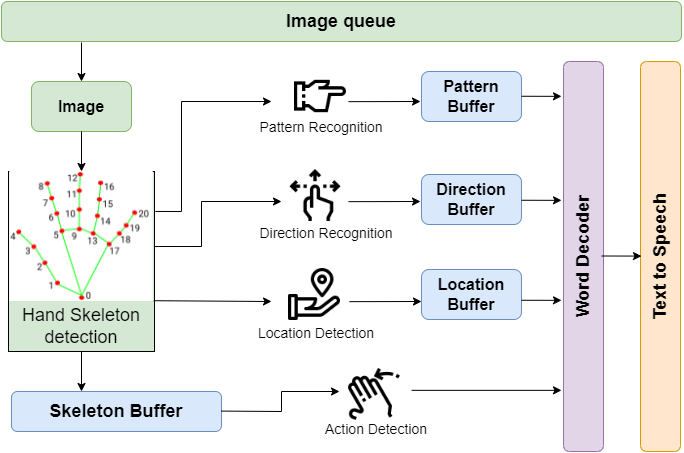
\includegraphics[width=0.9\textwidth]{img/Chap4/OverviewOfTheSystemModules-Old.png}
	\caption{Overview of the old system structure}
	\label{fig:Chap4-OverviewOfTheSystemModules-Old}
\end{figure}

Those six main modules mentioned above are the ones we planned up at the beginning of this thesis. However, during the implementing period, we found it hard to build the action detection module, despite going through most of the modules. It is problematic due to its demands on the smartphone and server.

There are words in sign language that contain many continuously moving patterns. There are a few solutions to detect which action the hands are doing; the first way is sending the whole video the camera captured to the server to process. This way, however, requires a strong connection between the camera module, smartphone, and the server and puts stress on the physical devices (the camera and smartphone); as a result, those devices will get hot quickly and can be damaged somehow. Another way is to increase the frame rate to get the action, but this one can also stress those devices; Moreover, we must have an algorithm continuously processing and detecting the movements, which, we admit, is hard to achieve.

Therefore, we had to deprecate that module and change our method to get the correct Vietnamese word to resolve that problem. Instead of using a combination of the four modules, including the action detection module, it now only has three left: pattern, direction, and location. Furthermore, in the word decoder module, we apply a heuristic search algorithm known as beam search, which uses the result of the three modules to look up the word in the database and return it to us. We will discuss each module's role and how it works in section \ref{sec:DetailImplementation}.

\begin{figure}[H]
	\centering
	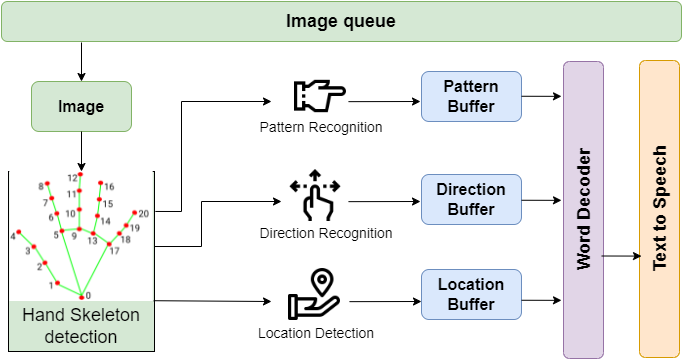
\includegraphics[width=0.9\textwidth]{img/Chap4/OverviewOfTheSystemModules-New.png}
	\caption{Overview of the new system structure}
	\label{fig:Chap4-OverviewOfTheSystemModules-New}
\end{figure}

\section{Detail Implementation}\label{sec:DetailImplementation}

\subsection{Hand pattern recognition}

Hand pattern recognition is the first and basic module of this system. While a person with disabilities does signs of sign language, his hands perform a series of different movements, where their hand may be spread out, clenched, or his fingers pointing out at something. Therefore, the role of this module is to recognize the pattern of the hands. Then combining the outcome with other modules, the system can give out the final result.

This module uses the output of the hand landmark model, which is a matrix size of 21. After calculating all the values in that matrix, we get a new matrix representing the distance between those 21 coordinates. Using the distance matrix as the input of CNN with the designed structure (see Figure \ref{fig:Chap4-StructureOfConvolutionalNeuralNetwork}), as seen in Figure \ref{fig:Chap4-OverviewOfTheSystemModules-New}, will tell us the pattern of the hand at the moment it is captured.

\begin{figure}[H]
	\centering
	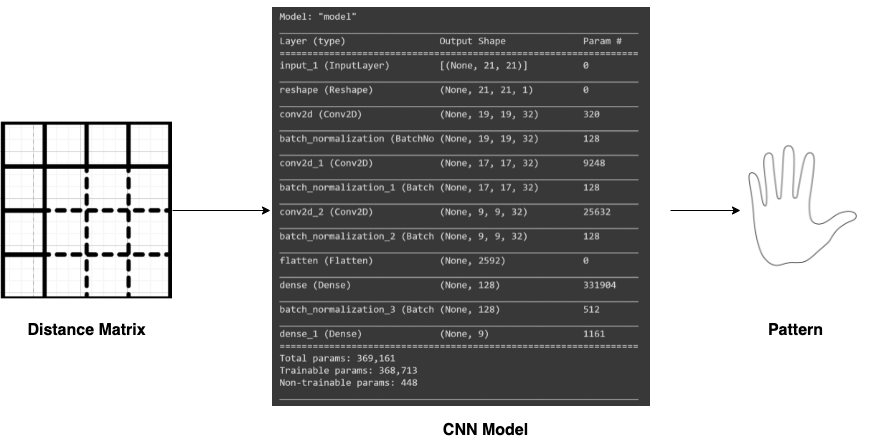
\includegraphics[width=\textwidth]{img/Chap4/Hand-Pattern-Reg-Model.png}
	\caption{Hand Pattern Recognition Pipe Line}
	\label{fig:Chap4-StructureOfConvolutionalNeuralNetwork}
\end{figure}

\subsection{Direction determination}

The directions of the hand include four directions, i.e., right, left, up, down, front, and back. Each hand's pattern combined with different directions leads to a different meaning. For example, the pattern that points at someone means the word "you"; on the other hand, when we point at ourselves, it means the word I (see Figure \ref{fig:Chap4-WordYouInSignLanguage} and Figure \ref{fig:Chap4-WordIInSignLanguage}).

\begin{figure}[H]
	\centering
	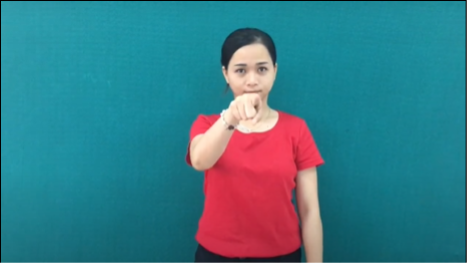
\includegraphics[width=0.6\textwidth]{img/Chap4/WordYouInSignLanguage.png}
	\caption{Word "You" (bạn) in sign language}
	\label{fig:Chap4-WordYouInSignLanguage}
\end{figure}

\begin{figure}[H]
	\centering
	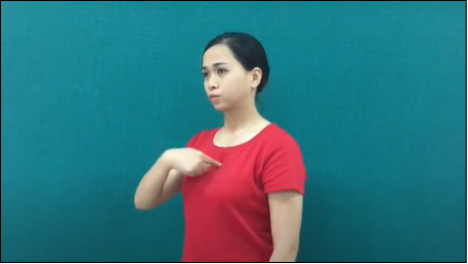
\includegraphics[width=0.6\textwidth]{img/Chap4/WordIInSignLanguage.png}
	\caption{Word "I" (tôi) in sign language}
	\label{fig:Chap4-WordIInSignLanguage}
\end{figure}

To determine the hand's direction, we use the hand landmark model provided in MediaPipe (see section \ref{sec:MediaPipe}). The inception here is that we calculate the distance between the tip of the index finger and the wrist, which can be called \textbf{vector(0, 8)}, then project it to the axis Ox, Oy, Oz, respectively. After that, we take each of those coordinates and compare them with the others. Finally, the one with the immense value will tell which axis the hand is on; besides, with the direction from the wrist to the tip of the index finger projected on that corresponding axis, we will know which direction the hand is.

\begin{figure}[H]
	\centering
	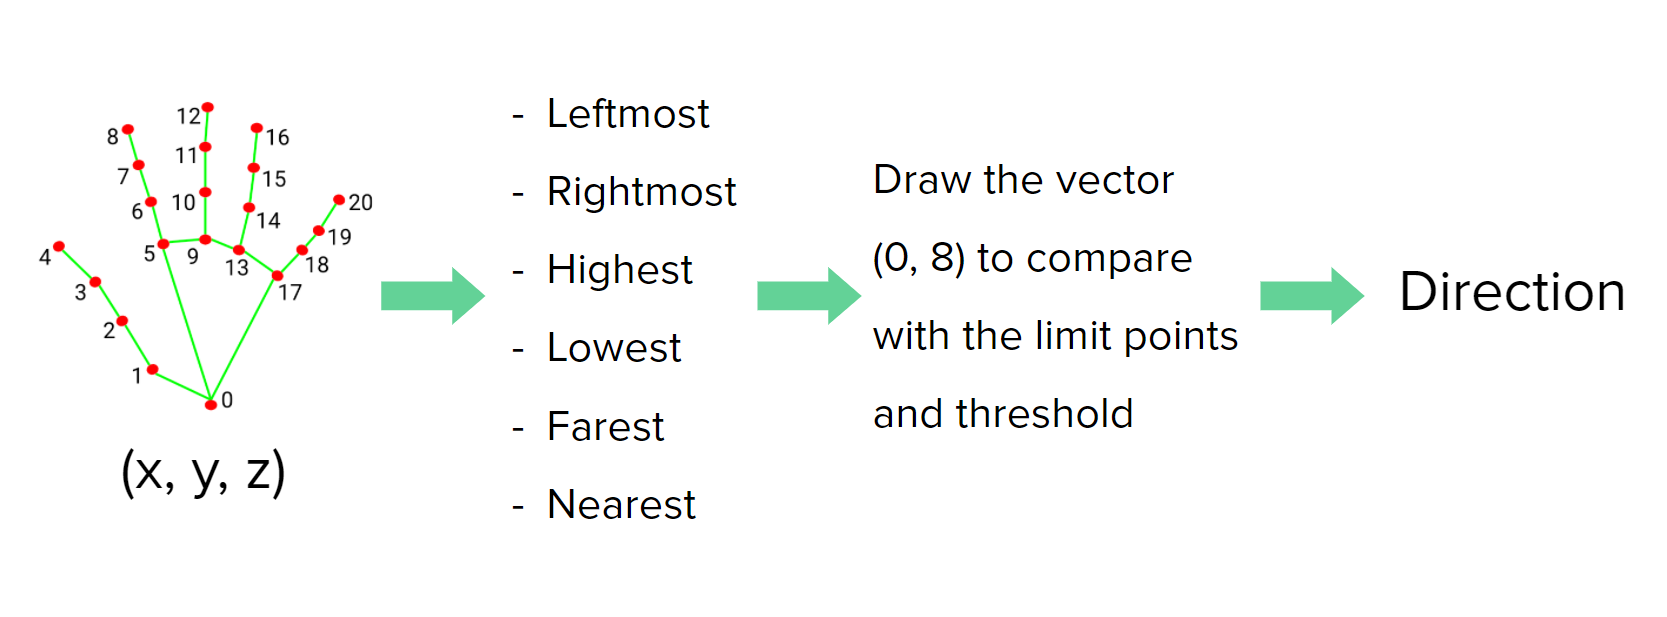
\includegraphics[width=\textwidth]{img/Chap4/DirectionSteps.png}
	\caption{Steps to detect the direction of the hand}
	\label{fig:Chap4-DirectionSteps}
\end{figure}

For instance, a hand is known to be pointing toward the left direction. The value of the distance, when projected on the axis Ox, will be the biggest one among the three projected values. Then, calculate the vector drawn from the wrist to the tip of the index finger; we will know the direction of the hand itself.

\begin{figure}[H]
	\centering
	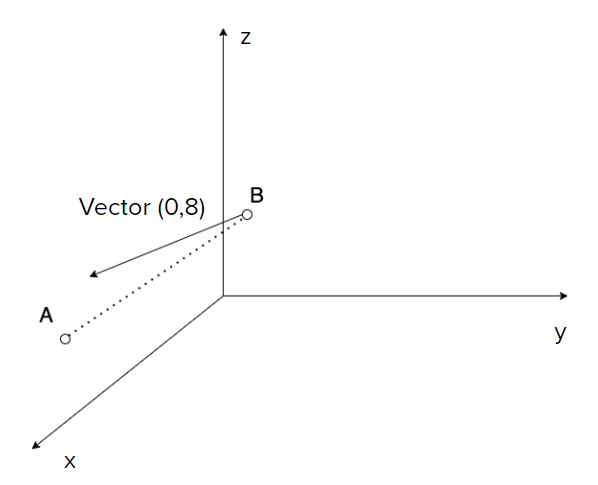
\includegraphics[width=0.6\textwidth]{img/Chap4/vector0-8-forwardLeft.png}
	\caption{Vector(0, 8) represent the hand pointing toward the left}
	\label{fig:Chap4-vector0-8-forwardLeft}
\end{figure}

\subsection{Location detection}

Locations of hand vary, is the hand put at forehead, mouth or the chest level, and so on. Every hand pattern that goes with every location will result in different words. Nevertheless, it is hard for the AI to know the hand's coordinates with only one camera, and its view is from above (see Figure \ref{fig:Chap4-ViewFromCamera}). However, we came up with some solutions to this issue.

The zooming method is the first approach we use to detect the hand location. In this solution, we will take images of the hand and calculate the size of the hand in every frame in order to know whether that hand is getting larger or smaller. Hence, if that hand is smaller than before, it means the hand is getting far away from the camera, and its location is somewhere at the chest level or the stomach level. Otherwise, the hand's location is nearer to the camera, at the mouth, nose, or forehead level.

\begin{figure}[H]
	\centering
	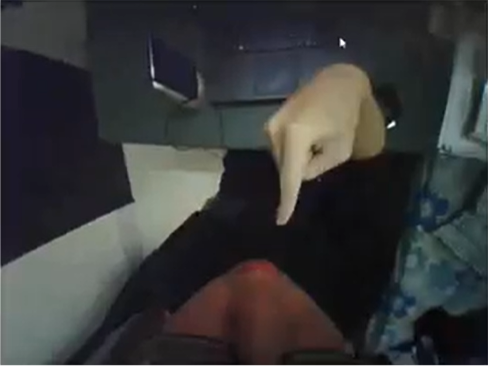
\includegraphics[width=0.6\textwidth]{img/Chap4/ViewFromCamera.png}
	\caption{View from the camera module}
	\label{fig:Chap4-ViewFromCamera}
\end{figure}

Nonetheless, the above solution still has an issue: every man's hand has a different size, and the system does not know the correct position of the hand. Therefore, another solution is to use a wide-angle camera and set it away from the forehead. With this solution, the camera can have a much broader view. Yet, since we only have a normal-angle camera, we could not try out this solution and confirm its suitability.

Another solution to detect the hand's location is using an ultrasonic sensor. In short, this sensor is an instrument that measures the distance to an object using ultrasonic sound waves (see Figure \ref{fig:Chap4-UltrasonicSensorFunction}). It works by emitting a sound wave with a frequency above the human hearing range. The sensor's transducer functions as a microphone, receiving and transmitting ultrasonic sound. The sensor measures the time between sending and receiving an ultrasonic pulse to determine the distance to a target.

\begin{figure}[H]
	\centering
	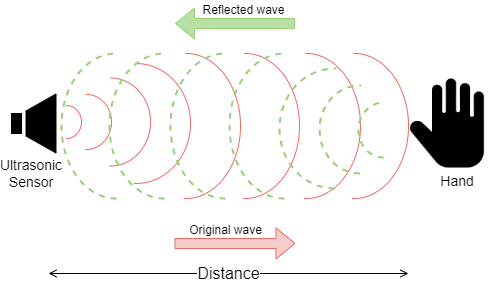
\includegraphics[width=0.7\textwidth]{img/Chap4/UltrasonicSensorFunction.png}
	\caption{Illustration of how the ultrasonic sensor works}
	\label{fig:Chap4-UltrasonicSensorFunction}
\end{figure}

\begin{wrapfigure}{r}{0.475\textwidth}
  \begin{center}
  	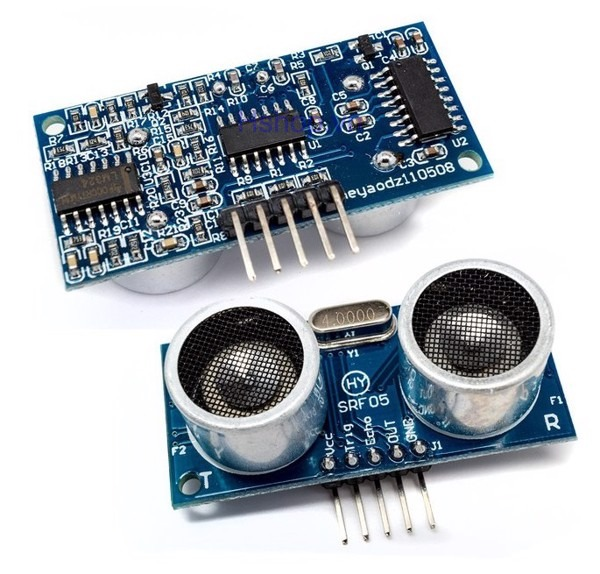
\includegraphics[width=0.3\textwidth]{img/Chap4/UltrasonicSensor.jpeg}
  \end{center}
	\caption{The ultrasonic sensor HY-SRF05}
  \label{fig:Chap4-UltrasonicSensorHYSRF05}
\end{wrapfigure}

In the thesis, the one we use for this module is the ultrasonic sensor HY-SRF05 (Figure \ref{fig:Chap4-UltrasonicSensorHYSRF05}), which is relatively cheap and meets our demand in measuring the distance between the camera and the hand. According to the retailer, the wide-angle this sensor can scan is up to 15 degrees. Moreover, its scanning range is between 2 cm and 450 cm, with the relative error fluctuating around 0.3 cm. Besides, the most accurate measurement distance is under 100 cm, which is more than enough when it comes to measuring from the forehead to the user's waist.


Consequently, after getting the result from the ultrasonic sensor of this location module, we put it within a hand state. And we will discuss how that hand state will help us translate sign language into Vietnamese in the following section.

\subsection{Word decoder}
% TODO:   Previous approach 

% [x] How to map word ?

% TODO:   New approach

% [x] Punish function

% [x] Using beam search

% [x] CTC decode

% [x] Flow

% [x] Expected result

% [...] Difficult and proposed solution

% [...] Dịch sang tiếng anh

% [...] Thêm các hình ảnh


% TODO: With previous approach

As discussed above, there are considerable technical difficulties in implementing the action detection module. We did some research and proposed a new model to resolve these problems. As a result, this change affects the word decoder module, which needs some adjustments.

The previous model decodes a word into four factors: pattern, location, direction, and action. After getting the outputs from the four modules, it will search the database to find the corresponding word. Figure \ref{fig:Chap4-MapWord} illustrates how an input containing four factors is mapped to the correct word in the database. Applying a basic searching algorithm, we have the system find the most appropriate word. If it can not find any, it will replace or deprecate some parts of the input and try again to find another word. After decoding and finding the suitable word, the application will display that word on the screen.

\begin{figure}[H]
	\centering
	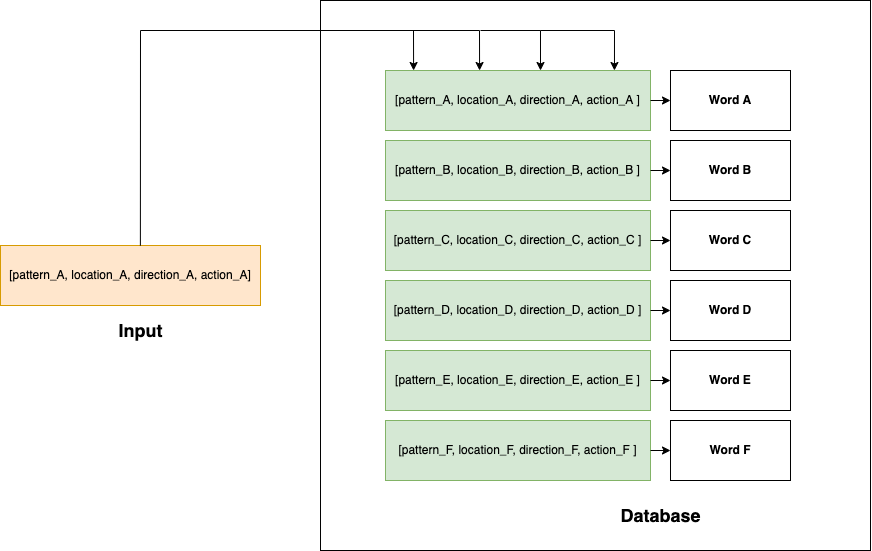
\includegraphics[width=\textwidth]{img/Chap4/MapWord.png}
	\caption{Map one to one data from four component with word in database and get result}
	\label{fig:Chap4-MapWord}
\end{figure}

\subsubsection{ Introduction to handstate }

Right after the deprecation of the action detection module, the question that comes up is how we can find the correct word without that module. Therefore, we propose a different model for a word that is not decoded into four factors like the previous model. It only contains three elements left: pattern, direction, and location. Consequently, each set of those three elements is called a hand state (\ref{fig:Chap4-HandState}), and a word is decoded into many different hand states.

This concept of hand state comes from the research of natural language processing, in which a word is composed of many characters. Accordingly, a word is concatenated from many hand states in this thesis. Then, we will get the desired word when going through the processing steps that we will discuss later in this proposal.

\begin{figure}[H]
  \centering
  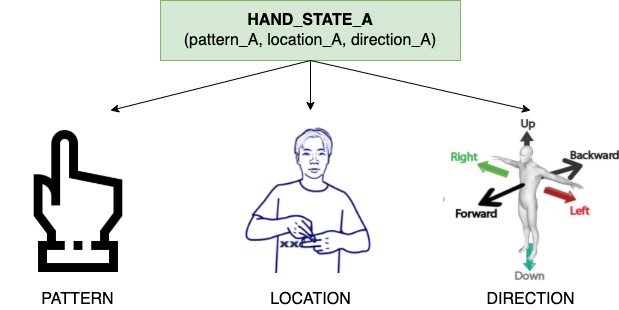
\includegraphics[width=0.6\textwidth]{img/Chap4/HandState.png}
  \caption{ Hand State which construct from pattern, location and direction}
  \label{fig:Chap4-HandState}
\end{figure}

\subsubsection{ Using beam search and CTC decode to map word}

After we have grasped the concept of hand state, we will come to the essential part of the model: converting the received hand states into words.
      
\begin{figure}[H]
  \centering
  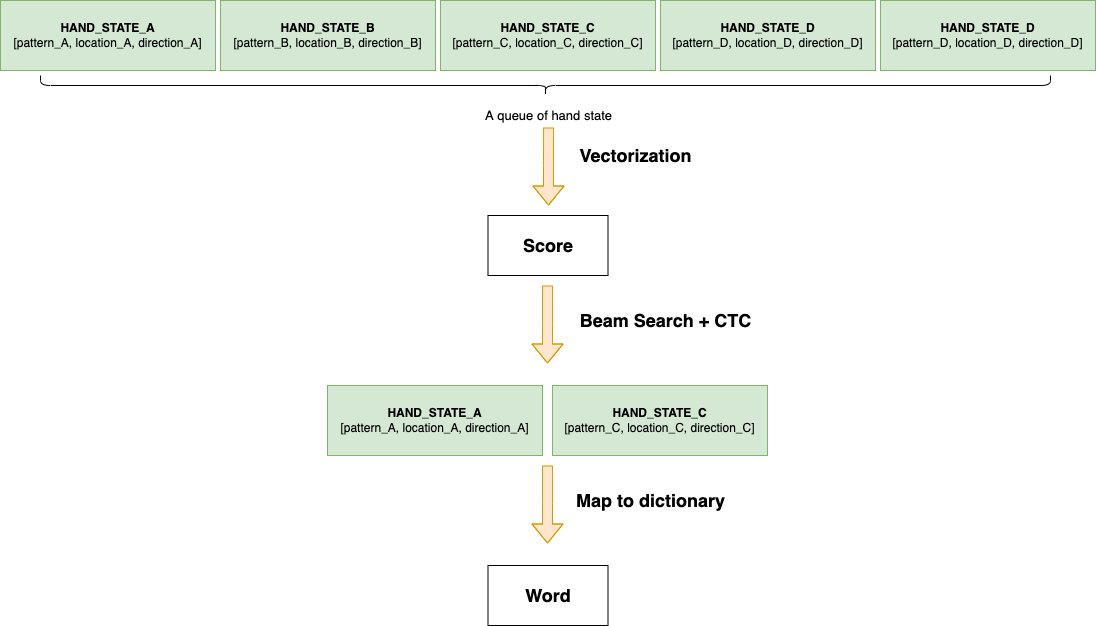
\includegraphics[width=\textwidth]{img/Chap4/Architechture.png}
  \caption{Architechture}
  \label{fig:Chap4-Architechture}
\end{figure}

Figure \ref{fig:Chap4-Architechture} is the model proposed by the authors for this section. The input will be a queue of hand states taken from the previous three components. Here, in our conventions, the queue length is set to 5, but it is not the final number, as we need more calculations and experimentation to find the right queue length. This model consists of three steps:

\begin{enumerate}
  \item \textbf{Vectorization:} This step converts a queue of many hand states \ref{fig:Chap4-HandStateQueue} into a matrix as input for beam search.
  \item \textbf{Beam search:} In this step, we will perform a beam search algorithm to choose which hand states are suitable for the input from the database. Besides, we propose using the CTC decode model to eliminate the wrong hand states or previous duplicated hand states, increasing the model's efficiency.
  \item \textbf{Map to the dictionary:} And finally, after going through the above two steps, from the initial queue, we will get the most likely hand states. Our job is to map these hand states to the database and find the correct word.
\end{enumerate}
      
\subsubsection{ Vectorization }
% TODO: Why we need punish
% TODO: how to perform -> Trình bày cách đánh giá như thế nào, cách trừ điểm và các phương châm đánh giá
% TODO: Sau khi punish dùng hàm softmax để chuyển các giá trị về dạng xác suất

When we get to this step, we get a queue of hand states. Because before entering the beam search module, we need a matrix representing the correlation between the outputs received from the components and the data in the database.

\begin{figure}[H]
  \centering
  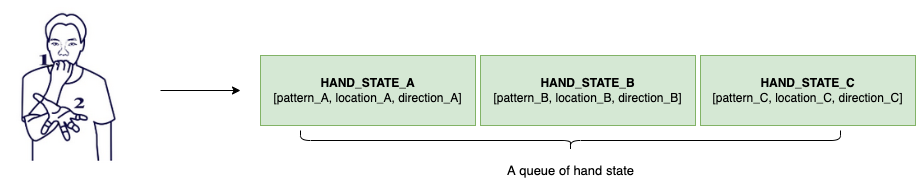
\includegraphics[width=\textwidth]{img/Chap4/HandStateQueue.png}
  \caption{A queue of hand state which get from three component in section ... }
  \label{fig:Chap4-HandStateQueue}
\end{figure}

From this queue, we will cycle through each hand state, compare it with the available hand state database, and evaluate the score for it based on the following principles \ref{fig:Chap4-Vectorization}:

\begin{enumerate}
  \item The score will be increased if the hand state matches the word in the database.
  \item Otherwise, the score will be decreased if that hand state does not match any.
\end{enumerate}

\begin{figure}[H]
  \centering
  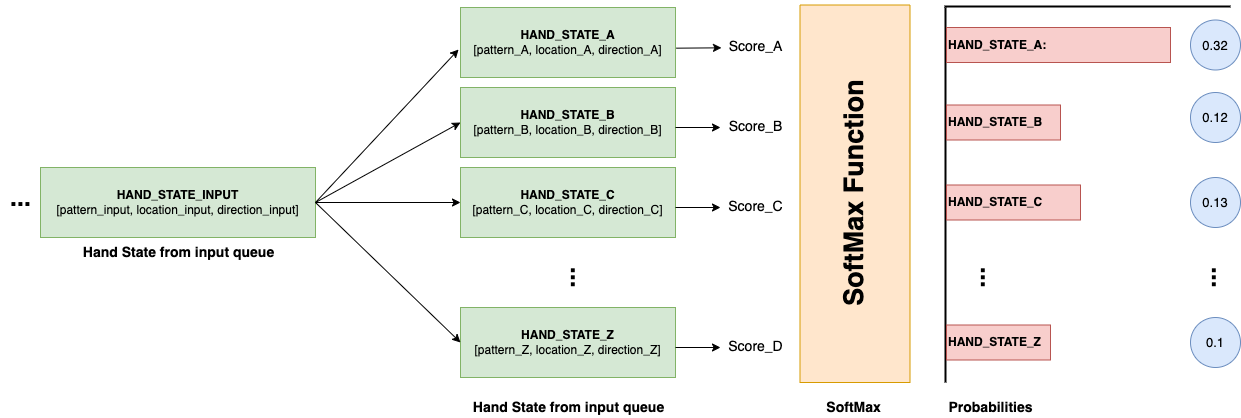
\includegraphics[width=\textwidth]{img/Chap4/Vectorization.png}
  \caption{ Vectorization }
  \label{fig:Chap4-Vectorization}
\end{figure}
% TODO: Change to Math
In the first principle, The more similarities the hand state retrieved from the queue has compared to that in the database, the higher it is scored. For example, in the database, we have a hand state as follows: 
$\begin{bmatrix}
  pattern \_ A & location \_ A & direction \_ A
\end{bmatrix}$
, and the hand state we get from the input is 
$\begin{bmatrix}
  pattern \_ A & location \_ A & direction \_ A
\end{bmatrix}$
then this hand state will be rated higher than the hand state 
$\begin{bmatrix}
  pattern \_ A & location \_ A & direction \_ B
\end{bmatrix}$
. And so on, we will, in turn, score the hand states taken from the queue.

On the second point, the minus point is evaluated based on its matching pattern with the hand states in the database. When the system recognizes patterns from the hand pattern recognition module (using the vision approach), it is likely to be wrong detected or mistaken. To resolve this problem and maximize the accuracy of the result, we put out a rule. With those patterns that are usually hard to detect, the minus point will be lower than simple ones. In short, the more complex the pattern to be recognized, the smaller the minus point is going to be.

% + Khi đánh giá các hand state, đối với trường hợp so trùng 2 pattern. Do các pattern này được nhận diện từ module hand pattern regconition (vision approach), do đó, sẽ có khả năng bị nhận diện bị sai, hoặc bị nhầm. Vì lẽ đó, để có thể đánh giá một cách chính xác và công bằng nhất có thể thì ở đây, đối với những pattern hay bị nhận diện sai, ta sẽ trừ điểm thấp và ngược lại, với những pattern đơn giản mà hệ thống lại nhận diện sai thì sẽ bị trừ điểm nhiều hơn.
      
After completing the above evaluation and scoring step, we will use a function to normalize the data (here, the authors use the softmax function) and return us a set of probabilities of the hand states in the row. Wait. We will use this set of probabilities as input for the beam search step.

\subsubsection{ Using beamsearch with CTC decode }
% TODO: Trình bày cách sử dụng beamsearch để tìm các cặp bộ 3
% TODO: Image beamsearch (get from ppt)
% TODO: Example
% TODO: Áp dụng CTC để handle một số trường hợp
% TODO: Các khó khăn gặp phải và hướng giải quyết

After passing the vectorization step, the hand states in our queue has been converted to a MxN matrix, where M is the length of the hand state's database and N is the length of queue.

By using beam search (\ref{fig:Chap4-BeamSearch}), we will get the most likely k hand state from the database. From the image below, we can imagine what happened later during beam search.

% Sau khi qua bước vectorizaion, các hand state trong hàng đợi của chúng ta
% đã được chuyển đổi thành một ma trận MxN với M là độ dài của cơ sở dữ liệu về
% các hand state và N là độ dài của hàng đợi.
      
% Bằng việc sử dụng beam search, từ sẽ thu được k hand state có khả năng nhất
% từ cơ sở dữ liệu. Từ hình ảnh bên dưới, ta có thể hình dung được những gì
% đã diễn ra sau trong quá trình thực hiện beam search

% FIXME: Insert image from ppt about matrix with beam search

\begin{figure}[H]
  \centering
  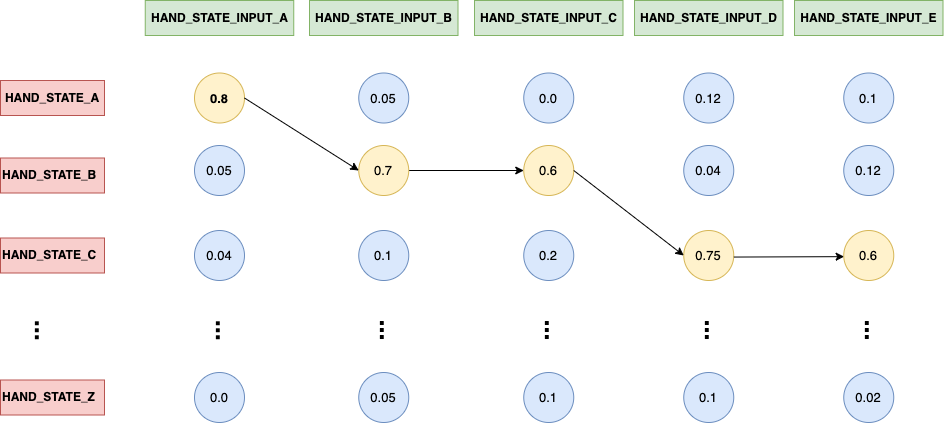
\includegraphics[width=\textwidth]{img/Chap4/BeamSearch.png}
  \caption{ Beam Search }
  \label{fig:Chap4-BeamSearch}
\end{figure}

However, as we can see that, after performing the beam search step, we will get a sequence of hand states whose length corresponds to the length of the input queue, these hand states can include duplicate hand states, or they can be wrong hand states. Therefore, we need to apply CTC algorithm to remove the hand states from infection. For the wrong hand states, in Vectorization step, we will set a threshold to discard these hand states and see it as a blank character. And after all step, after beam search CTC decode, we will get the desired result.

% Tuy nhiên, có thể thấy được rằng, sau khi thực hiện xong bước beamsearch,
% ta sẽ thu được một dãy các hand state có độ dài tương ứng với độ dài của hàng đợi
% , các hand state này có thể bao gồm những hand state bị trùng nhau, hoặc cũng có thể
% là những hand state bị sai. Do đó, ta cần áp dụng thêm CTC decode để loại bỏ các hand state
% bị trùng này. Đối với những hand state bị nhận sai từ những module trước thì ở bước Vectorization,
% ta sẽ đặt một threshold để loại bỏ những hand state này và xem như hand state đó là một ký tự rỗng (" ")
% và cuối cùng, sau khi áp dụng CTC decode vào, ta sẽ thu được kết quả mong muốn

% FIXME: Insert image about the result (get from ppt)

      
      
    \subsubsection{ Map to dictionary }
      % TODO: Cách map như thế nào

      \begin{figure}[H]
        \centering
        
\includegraphics[width=\textwidth]{img/Chap4/Result.png}
        \caption{ Map to dictionary and get word }
        \label{fig:Chap4-Result}
      \end{figure}

      % Sau khi nhận được một tập các hand state có khả năng nhất, việc còn lại là
      % chúng ta sẽ map vào cơ sở dữ liệu, như cách mà chúng ta đã làm trong mục ..., 
      % nhưng thay vì map với bộ 4 thành phần thì ở đây, ta sẽ map với input các hand state thu được
      % từ bước ... .
      % Và như thế, ta sẽ thu được từ vựng mà không cần phải dùng tới module action detection.
      After getting a set of most likely hand states, all that remains is for us to map to the database, as we did in section above, but instaed of map with 4-component set, in here, we will map with input retrieved from this previous step. And finally, we will get the word (\ref{fig:Chap4-Result}) without using the action detect module.



\subsection{Text-to-speech}

In addition, sometimes, people do not always read the result from the phone's screen, so to make it easier for them to know the answer after translating process, the application can speak it out loud. Basically, one way to do this is to build a database of many sound files mapped with the corresponding word in Vietnamese. This approach, however, is not efficient as it requires a massive effort in creating the database. We must record every single word and map them all together.

Instead of using that approach, we use a well-known speech service from Google called Text-to-speech. According to Google, Text-to-Speech converts text input into natural human speech audio data. And this service supports many languages, including the one that we need, Vietnamese. With the provided API from that speech service, our application can speak up the result without an extensive sound database in the user's phone.

In fact, this API is a freemium service. Text-to-Speech costs are determined by the number of characters transmitted to the service each month to be synthesized into audio. Google states on their website that,  "The first 1 million characters for WaveNet voices are free each month. For Standard (non-WaveNet) voices, the first 4 million characters are free each month. After the free tier has been reached, Text-to-Speech is priced per 1 million text characters processed." This thesis only needs the standard (non-WaveNet) plan, which provides us 4 million characters free each month and only costs USD 4.00 per following 1 million characters. In the upcoming phases of building up the application, the number that we will use is negligible compared to 4 million free characters. Therefore, we decided to apply this Text-to-speech module using Google service in this thesis.
% \chapter{Upcoming plan}

TL;DR: Discuss shortly about the result, what we did not achieve and overview of the upcoming plan.

\section{The camera module}

After having discussed mainly the solutions and implementations of the soft modules in the system, we must move on to the main one that is considered to be the eyes of this thesis, which is the camera module. This section will discuss what parts are in a camera module and represent some images of a real one we built.

We can easily find the camera modules' parts from any retailer selling electrical components, robots, and Arduino kits. Additionally, in the current era of e-commerce, it is easier for us to find and compare those components that we need online. The parts required to build a camera module are listed below.

First, we need a camera part, and ESP32-CAM is the perfect one for this role. It is inexpensive and easy to use, making it ideal for our thesis that requires complex functions like image tracking and recognition. Furthermore, it integrates Wi-Fi, traditional Bluetooth, which help us in sending the images to the user's smartphone for the next steps in translating sign language.

Secondly, we need a converter adapter to help us sideload the program into the camera module. Besides, the third part that we need is the ultrasonic sensor mentioned in the TK section. It plays a role in location detection, which will tell the system the distance between hands and the camera module. Last but not least, this camera module needs a battery to power the whole module, and we reckon that the volume of about 100 mAh is fine.

Furthermore, there must be a box to store all the above parts. With the help of current 3D printing technology, we design that package on Tinkercad, an online 3D modeling program that runs on the web browser. After getting all the necessary components, we tried to put them all together and get the result below.

\begin{figure}[H]
  \centering
  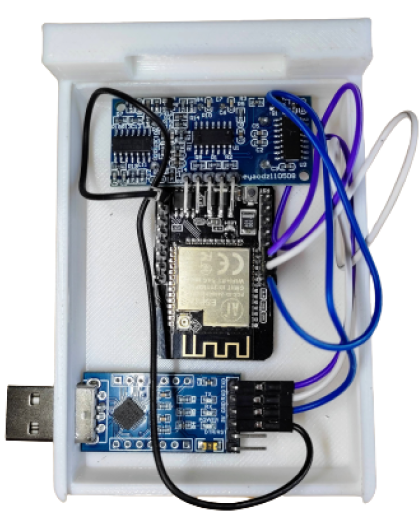
\includegraphics[width=0.45\textwidth]{img/Chap5/Prototype_View_inside.png}
  \caption{The components inside the camera module prototype}
\end{figure}

\begin{figure}[H]
  \centering
	\begin{subfigure}[b]{0.45\textwidth}
    \centering
    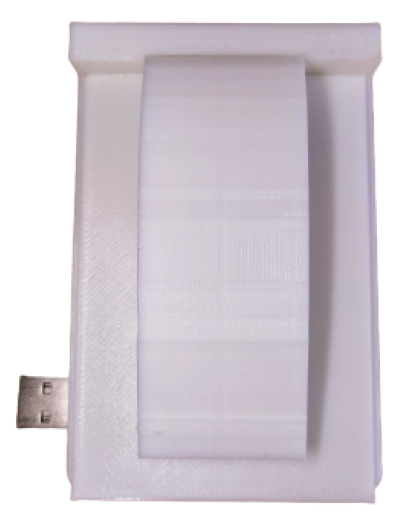
\includegraphics[width=\textwidth]{img/Chap5/Prototype_View_above.png}
  \end{subfigure}
  \hfill
	\begin{subfigure}[b]{0.46\textwidth}
    \centering
    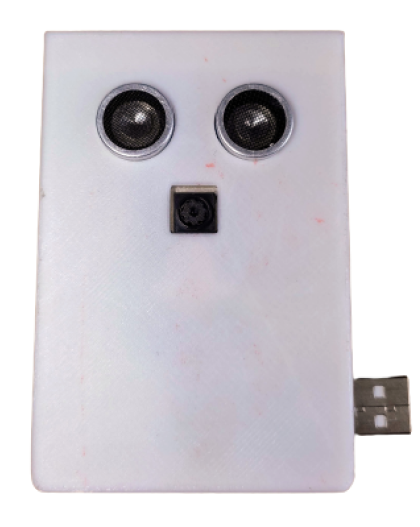
\includegraphics[width=\textwidth]{img/Chap5/Prototype_View_under.png}
  \end{subfigure}
	\caption{Views of the camera module prototype from the above and under}
\end{figure}

\begin{figure}[H]
  \centering
	\begin{subfigure}[b]{0.45\textwidth}
    \centering
    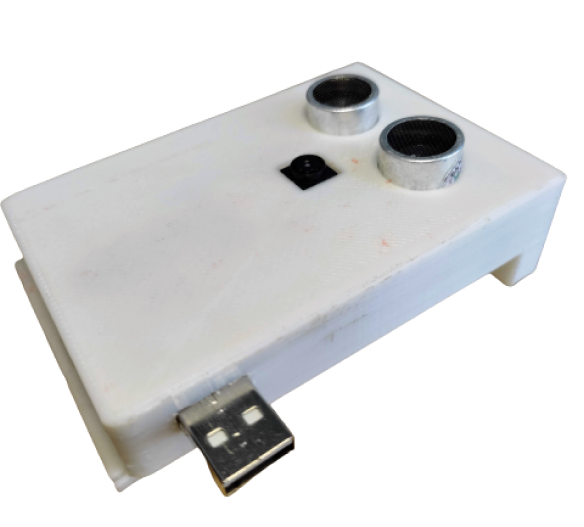
\includegraphics[width=\textwidth]{img/Chap5/Prototype_View_side_1.png}
  \end{subfigure}
  \hfill
	\begin{subfigure}[b]{0.45\textwidth}
    \centering
    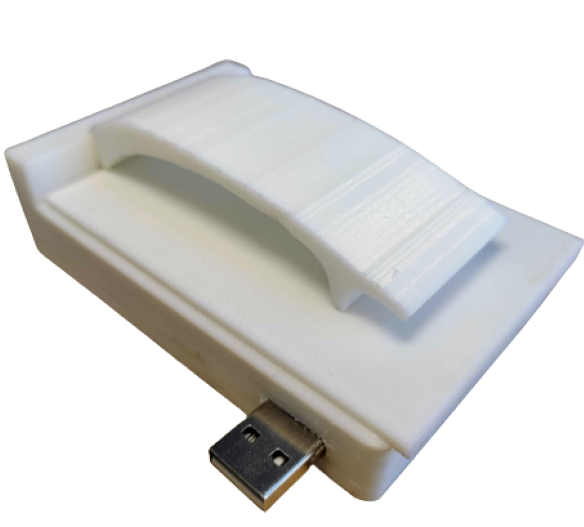
\includegraphics[width=\textwidth]{img/Chap5/Prototype_View_side_2.png}
  \end{subfigure}
	\caption{Views of the camera module prototype from the sides}
\end{figure}

Nevertheless, due to the smallest number that a 3D printer can print, the box's cover is a bit hard to put in. And the hanger that helped hang the box on the hat is not as flexible as we thought, so it needs a redesign.

\section{App design}

The application must satisfy user experience, and user interface demands. And during the research phase of this thesis, we did design a prototype for the application, including two more features besides the main one. Those features are a sign language dictionary and a learning system. We will talk more about those features in the later sections.

Before going through the design of this application, we must state that they do not cover all the screens needed for the application yet. And they are not the final design that we have. However, we have some conventions when designing this prototype, such as the corner is rounded and the colors are pale, not too bright, to make the users feel calm somehow and comfortable when using the application.

\begin{figure}[H]
  \centering
  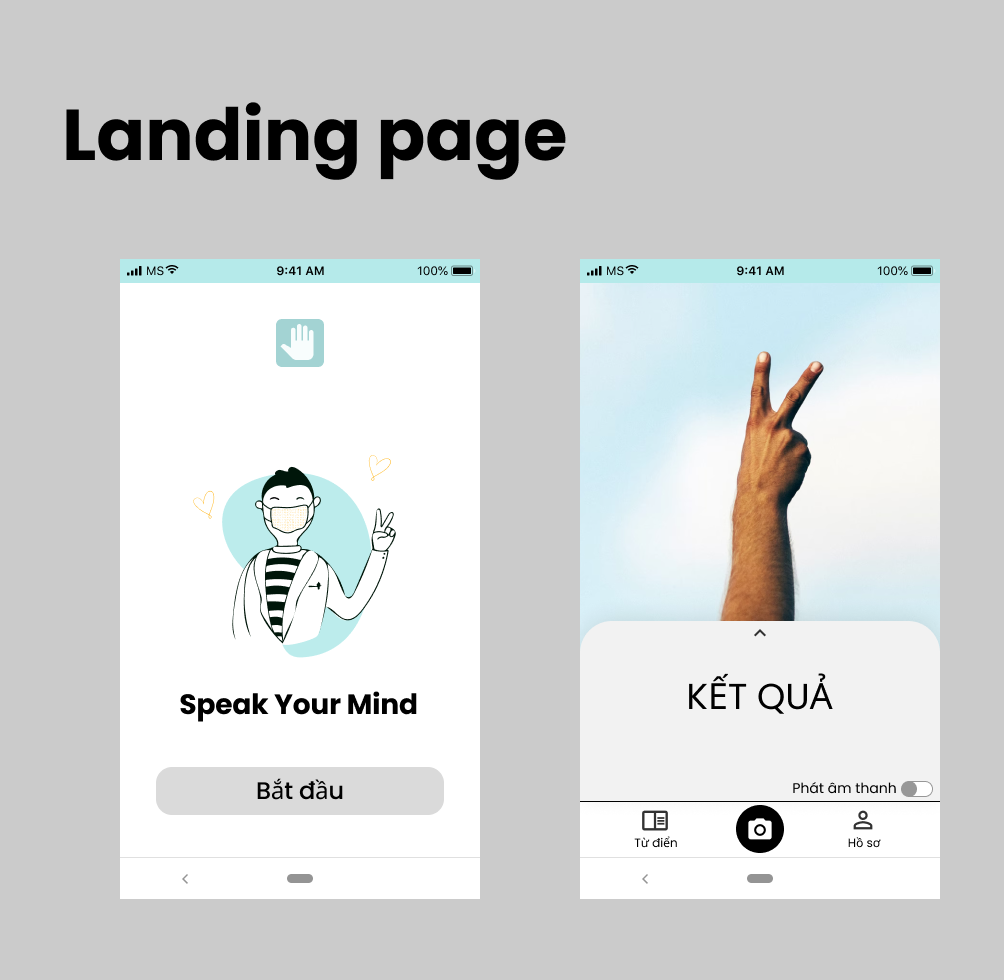
\includegraphics[width=0.8\textwidth]{img/Chap5/Landing_page.png}
  \caption{The landing page of the application}
\end{figure}

\begin{figure}[H]
  \centering
  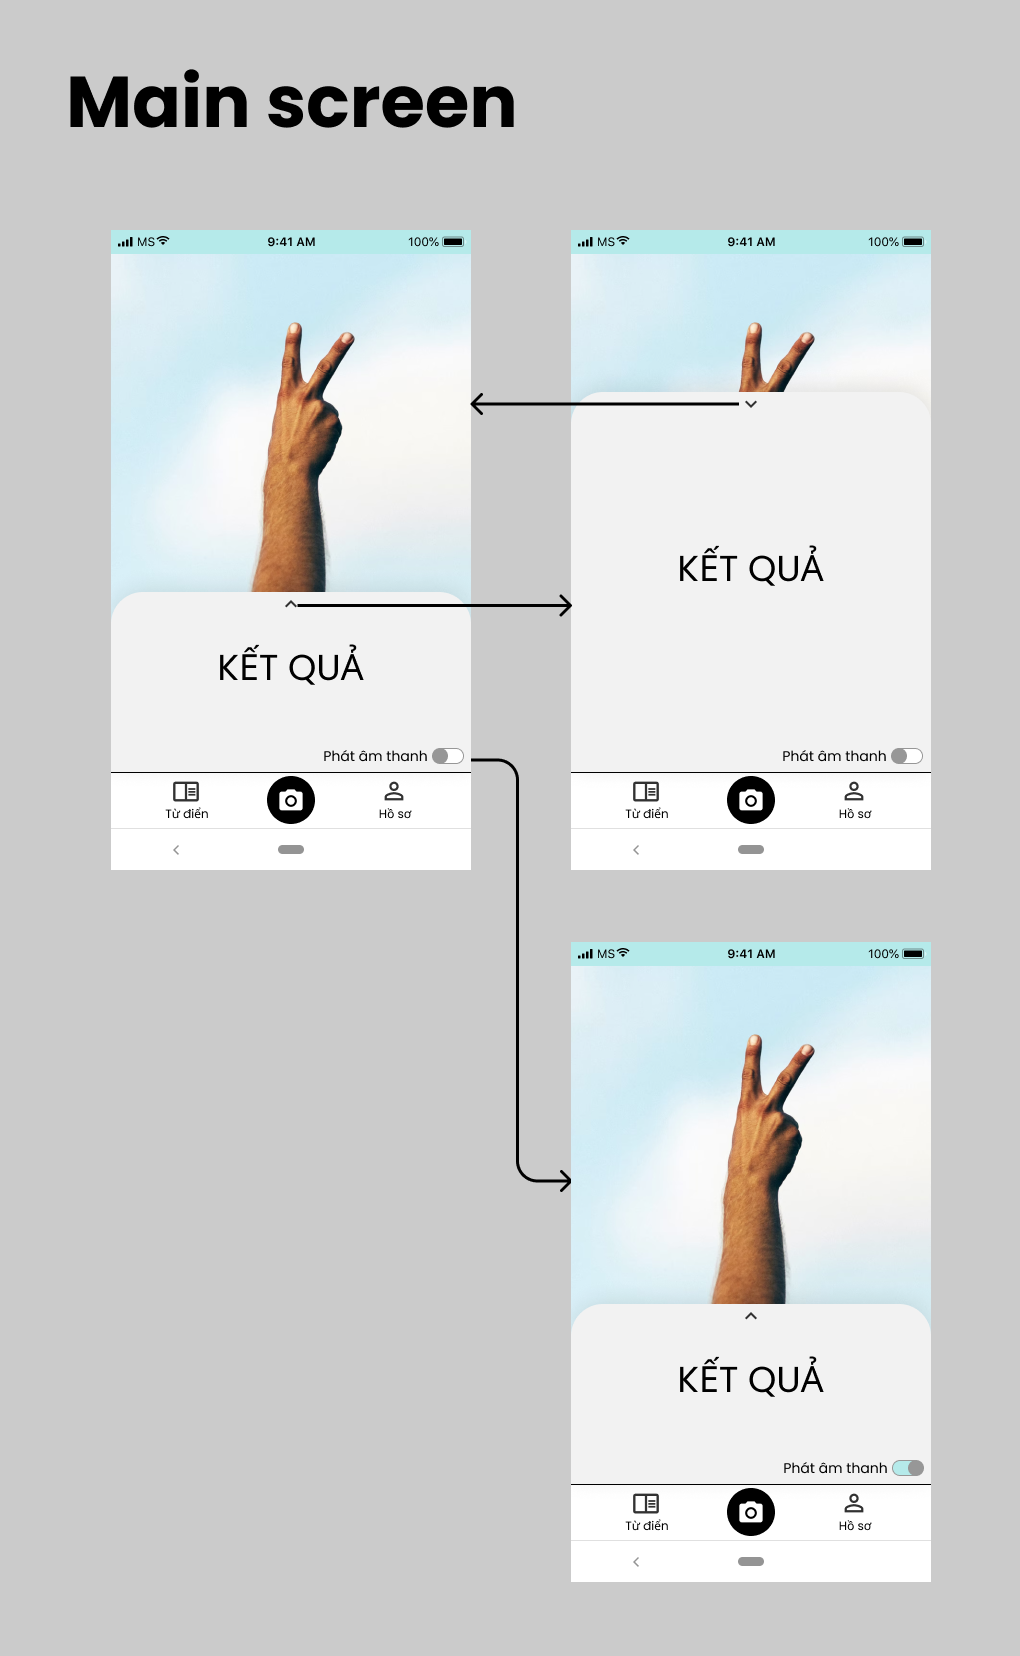
\includegraphics[height=0.8\textheight]{img/Chap5/Main_screen.png}
  \caption{The main screen of the application}
\end{figure}

\begin{figure}[H]
  \centering
  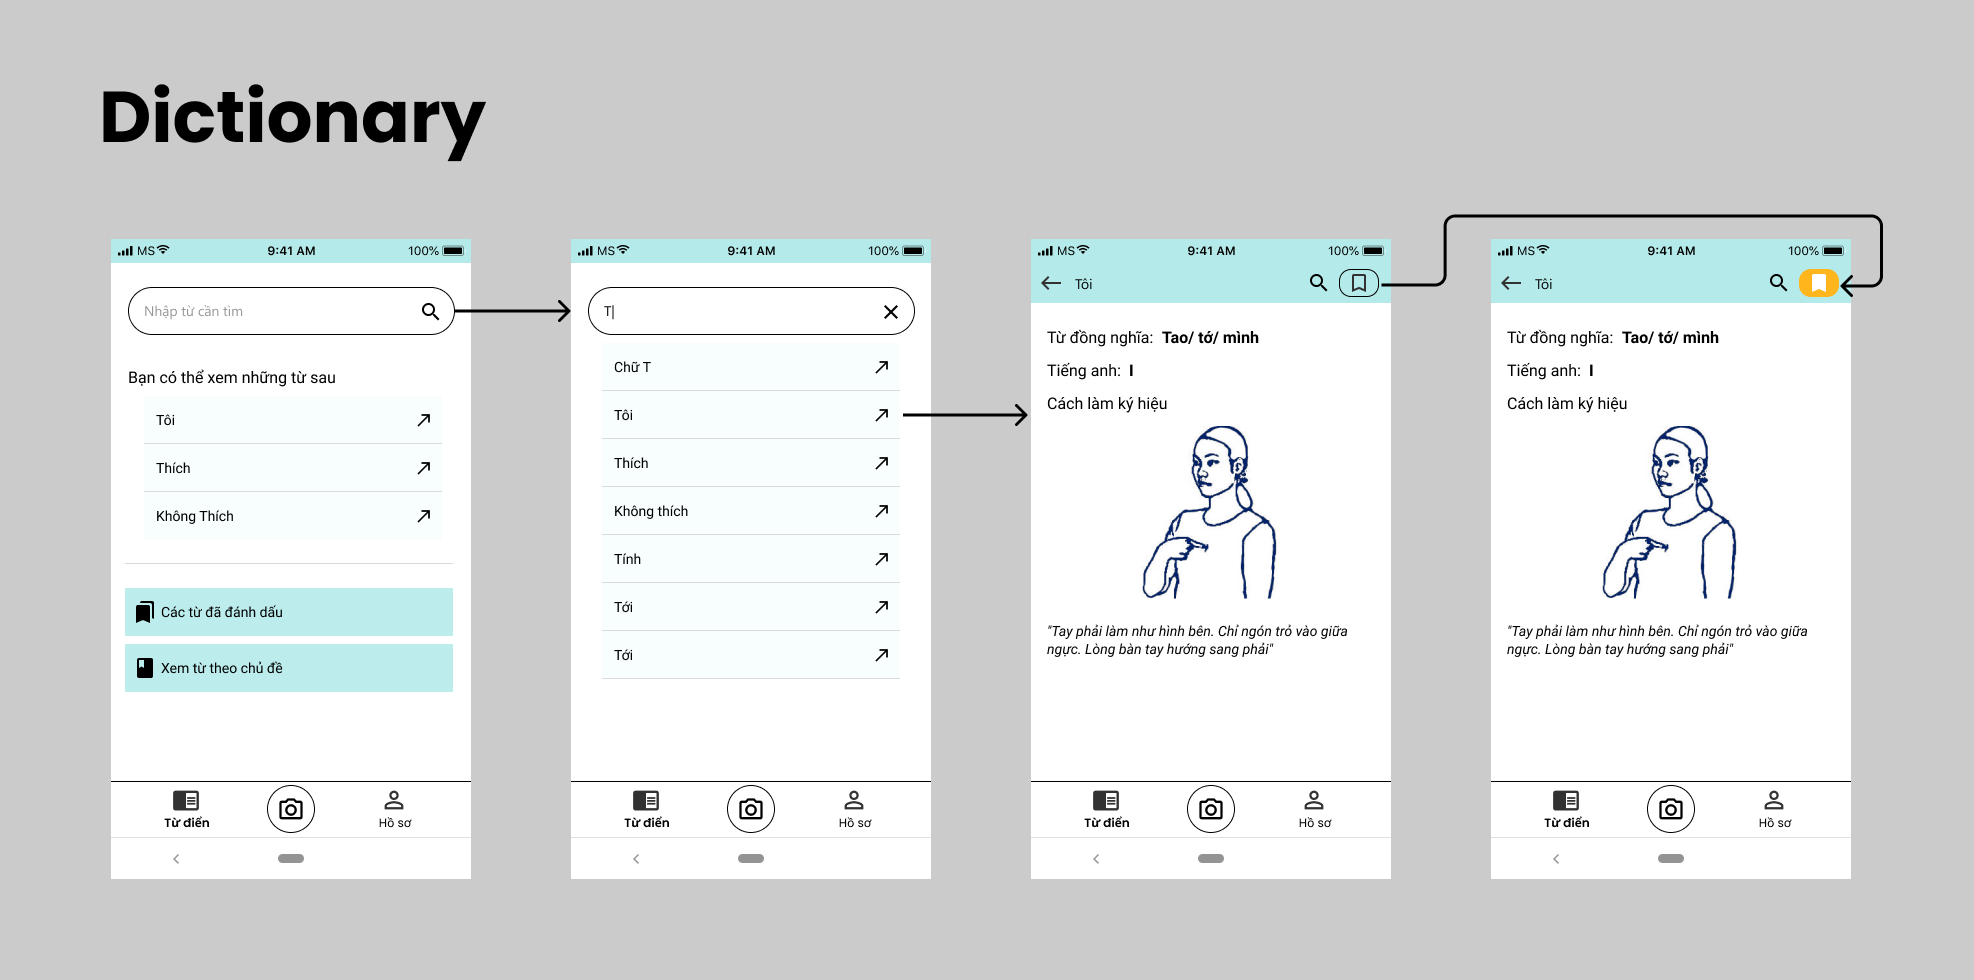
\includegraphics[width=\textwidth]{img/Chap5/Dictionary.png}
  \caption{The main screen of the application}
\end{figure}

\begin{figure}[H]
  \centering
  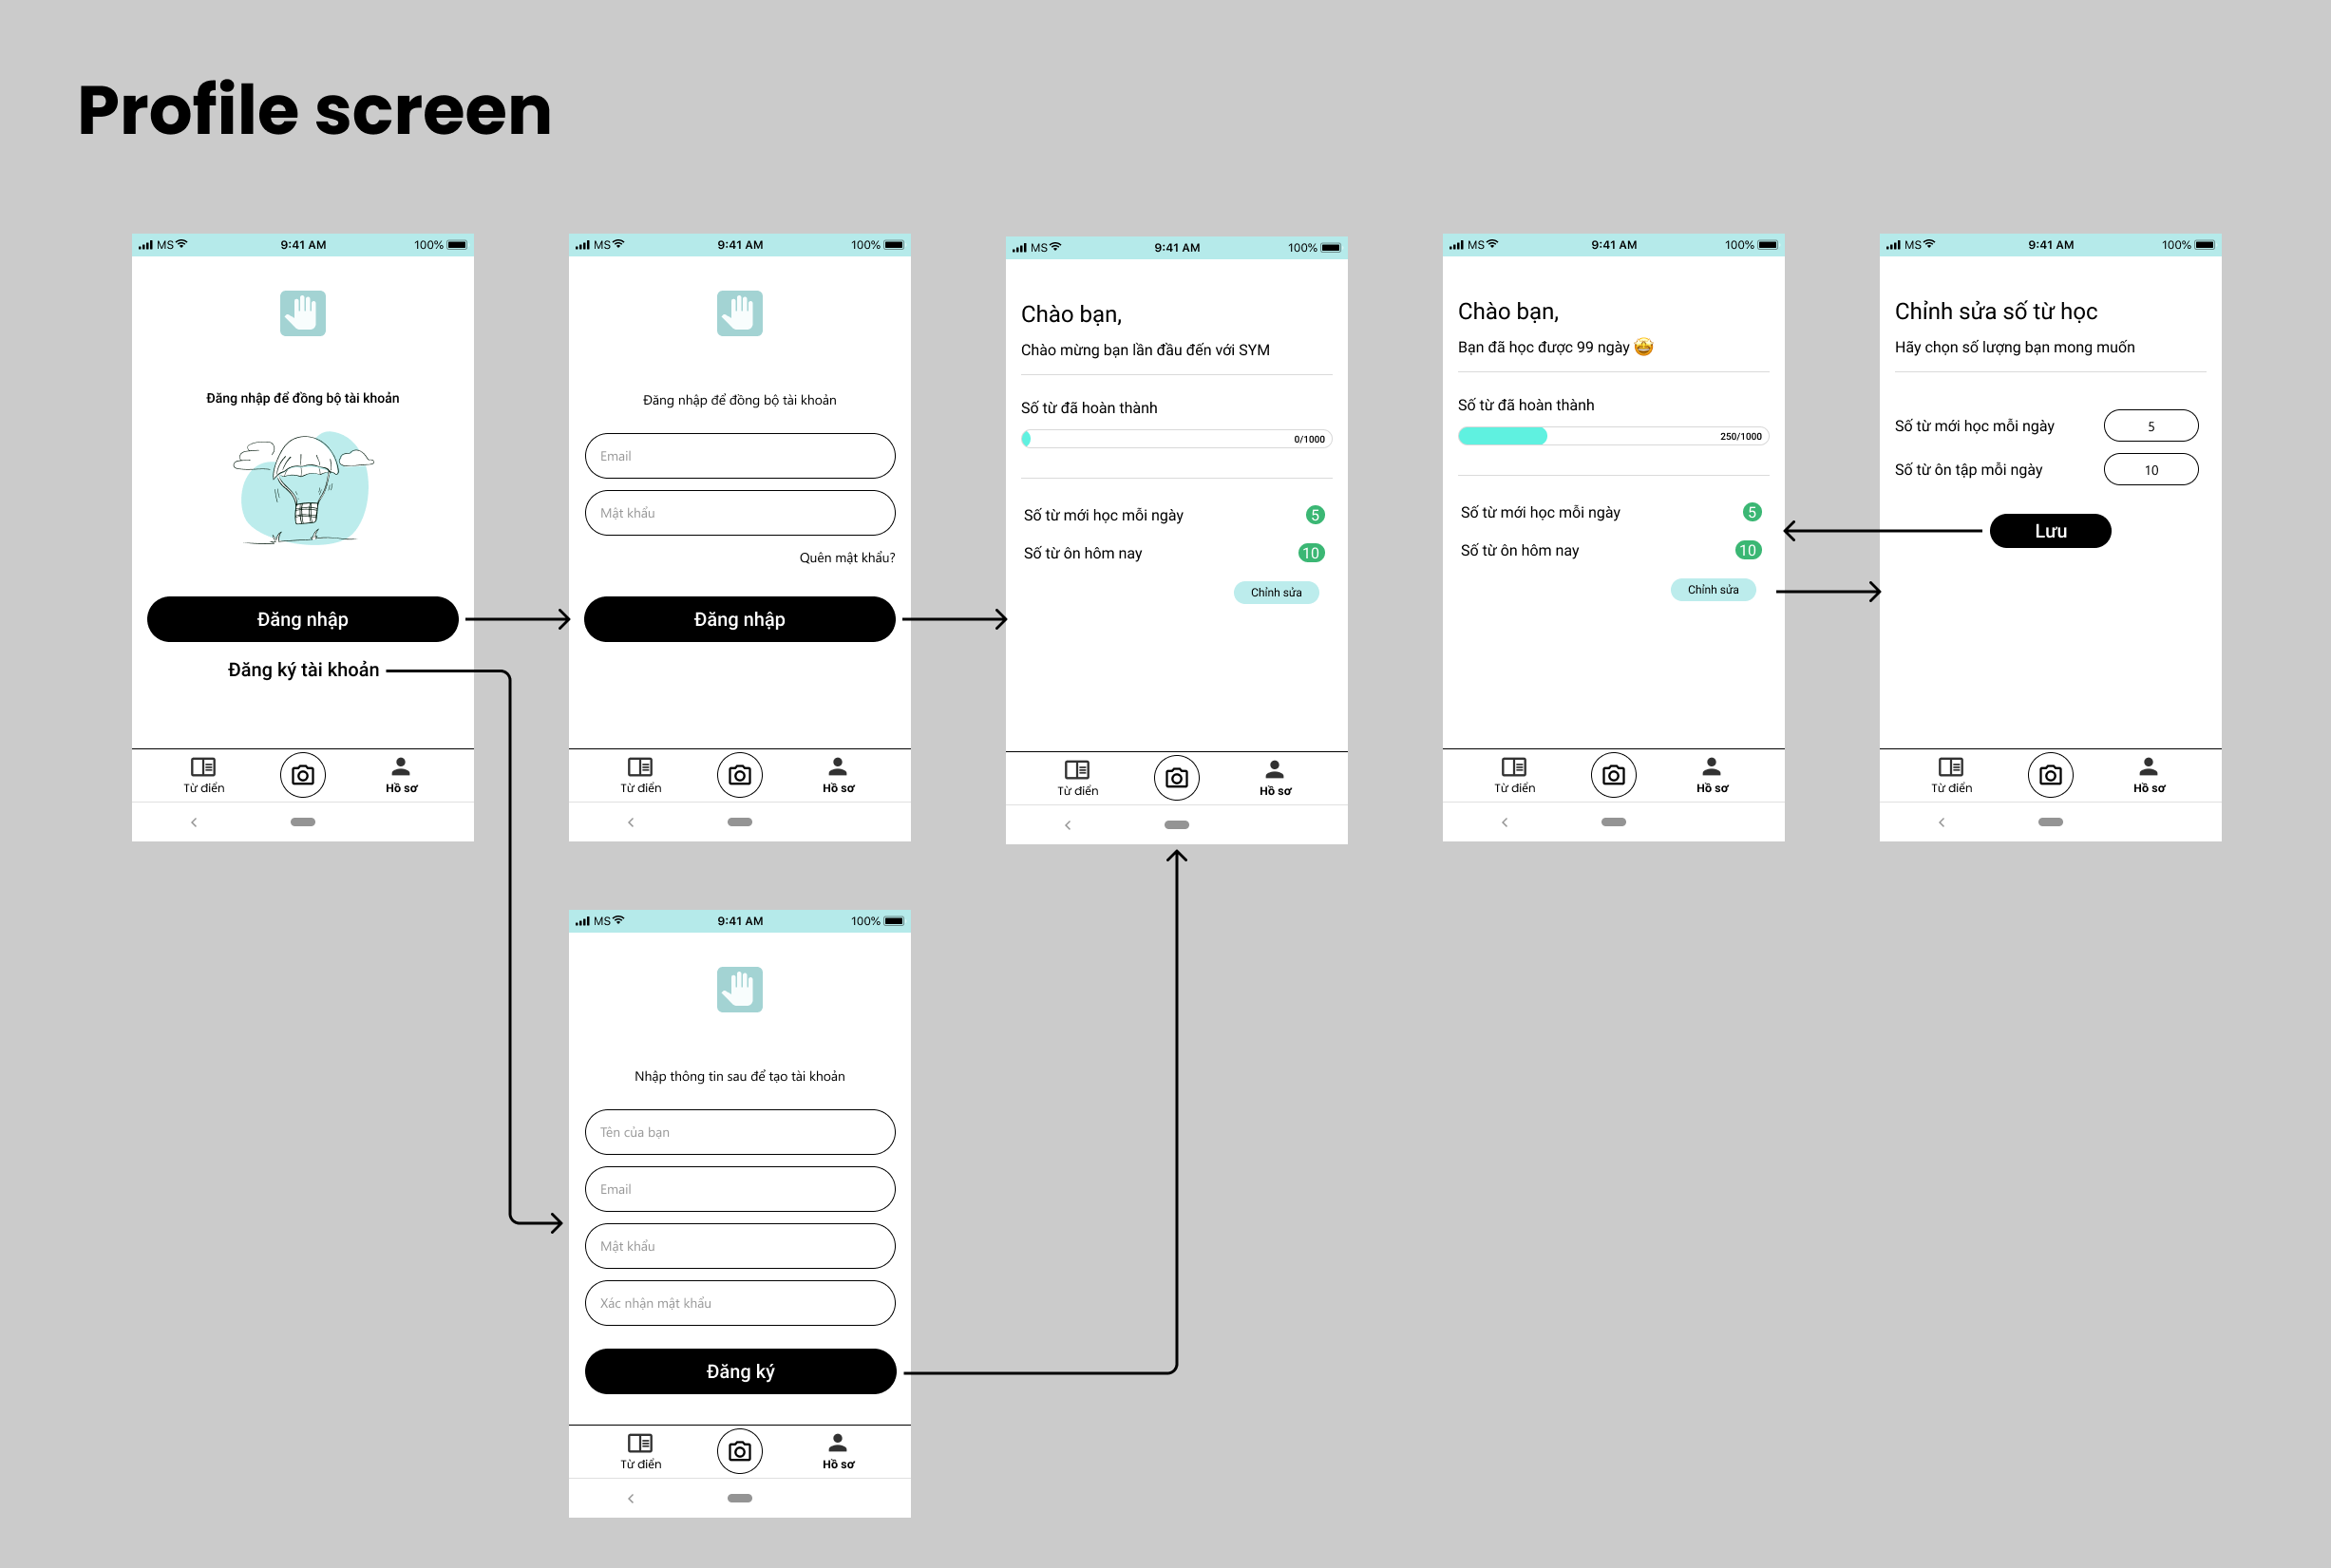
\includegraphics[width=\textwidth]{img/Chap5/Profile_screen.png}
  \caption{The main screen of the application}
\end{figure}

\section{New features and plan for thesis}

To expand the group of people using this application, we will implement additional features into the main application to help ordinary people learn and know more about sign language. Those features are a sign language dictionary and a learning system that help people learn sign language more efficiently.

\begin{itemize}
  \item \textbf{Sign language dictionary:} like any other dictionary, but dictionary has another element, which is containing the videos to illustrate the sign of the words.
  \item \textbf{Learning system:} apply the spaced repetition technique, which help people learn much faster and more efficient.
\end{itemize}

% \input{chapter/chapter6-proposedThesisChapters.tex}
\chapter{Implementation}

\chapter*{Result and evaluation}


\chapter{Summary}

This thesis applies image processing and artificial intelligence, whose purposes are to research and build a system that can translate sign language into Vietnamese using only a camera module and a smartphone.

So far, a sign language translating system has been a massive challenge to many scientists and engineers because of the complexity of sign language and the diversity of the way people use it around the world. Moreover, when we researched and built the system, there were a few similar systems, but they only translated the sign language alphabet.

In addition, talking about human values, this system can resolve the lack of sign-language translators in Vietnam. It, indeed, means that people having disabilities will have the chance to live, work and communicate like those who do not. They can have a better education as the teacher can understand their thoughts and connect more efficiently. They can have better health as the health force has the chance to know more about how they are, what they feel, which means we can provide them a better treatment for their problem. Their life will be easier as the surrounding people can get them and talk to them more clearly.

The deaf and mute are also a part of this world, a part of us, not apart from us. Therefore, we firmly believe the deaf and mute deserve to have the chance to speak up, be heard, be seen, and be acknowledged. With this application, we people can know each other and communicate fluently regardless of our level of knowledge of sign language. Ultimately, our bonds will grow more vital and more profound, which will lead to a better world for the entire human race.

Those human values emphasize the importance of this project in our world. Besides, the promising solution we presented throughout this proposal means it is possible to translate sign language with the current technologies. In the upcoming time, we have more resources to dedicate our time to completing our algorithm, which results in the higher accuracy of the translation process and completing the thesis thoroughly.


\newpage
%-	Danh mục TL tham khảo
%-	Phụ lục (nếu có)
\bibliographystyle{plain}
\bibliography{refs}

\end{document}